% Options for packages loaded elsewhere
\PassOptionsToPackage{unicode}{hyperref}
\PassOptionsToPackage{hyphens}{url}
\PassOptionsToPackage{dvipsnames,svgnames,x11names}{xcolor}
%
\documentclass[
  11pt,
  bookmarksnumbered]{article}
\usepackage{amsmath,amssymb}
\usepackage{lmodern}
\usepackage{iftex}
\ifPDFTeX
  \usepackage[T1]{fontenc}
  \usepackage[utf8]{inputenc}
  \usepackage{textcomp} % provide euro and other symbols
\else % if luatex or xetex
  \usepackage{unicode-math}
  \defaultfontfeatures{Scale=MatchLowercase}
  \defaultfontfeatures[\rmfamily]{Ligatures=TeX,Scale=1}
\fi
% Use upquote if available, for straight quotes in verbatim environments
\IfFileExists{upquote.sty}{\usepackage{upquote}}{}
\IfFileExists{microtype.sty}{% use microtype if available
  \usepackage[]{microtype}
  \UseMicrotypeSet[protrusion]{basicmath} % disable protrusion for tt fonts
}{}
\makeatletter
\@ifundefined{KOMAClassName}{% if non-KOMA class
  \IfFileExists{parskip.sty}{%
    \usepackage{parskip}
  }{% else
    \setlength{\parindent}{0pt}
    \setlength{\parskip}{6pt plus 2pt minus 1pt}}
}{% if KOMA class
  \KOMAoptions{parskip=half}}
\makeatother
\usepackage{xcolor}
\usepackage[margin=1in]{geometry}
\usepackage{longtable,booktabs,array}
\usepackage{calc} % for calculating minipage widths
% Correct order of tables after \paragraph or \subparagraph
\usepackage{etoolbox}
\makeatletter
\patchcmd\longtable{\par}{\if@noskipsec\mbox{}\fi\par}{}{}
\makeatother
% Allow footnotes in longtable head/foot
\IfFileExists{footnotehyper.sty}{\usepackage{footnotehyper}}{\usepackage{footnote}}
\makesavenoteenv{longtable}
\usepackage{graphicx}
\makeatletter
\def\maxwidth{\ifdim\Gin@nat@width>\linewidth\linewidth\else\Gin@nat@width\fi}
\def\maxheight{\ifdim\Gin@nat@height>\textheight\textheight\else\Gin@nat@height\fi}
\makeatother
% Scale images if necessary, so that they will not overflow the page
% margins by default, and it is still possible to overwrite the defaults
% using explicit options in \includegraphics[width, height, ...]{}
\setkeys{Gin}{width=\maxwidth,height=\maxheight,keepaspectratio}
% Set default figure placement to htbp
\makeatletter
\def\fps@figure{htbp}
\makeatother
\setlength{\emergencystretch}{3em} % prevent overfull lines
\providecommand{\tightlist}{%
  \setlength{\itemsep}{0pt}\setlength{\parskip}{0pt}}
\setcounter{secnumdepth}{5}
\usepackage{titling}
\usepackage{pdfpages}
\usepackage{tocloft}
\usepackage{amsmath}
\usepackage{atbegshi}% http://ctan.org/pkg/atbegshi
\AtBeginDocument{\AtBeginShipoutNext{\AtBeginShipoutDiscard}}
\usepackage[spanish]{babel}
\usepackage{csquotes}
\usepackage{setspace}
\usepackage{float}
\floatplacement{figure}{H}
\usepackage[T1]{fontenc}
\usepackage[utf8]{inputenc}
\usepackage{fancyhdr}
\usepackage{hanging}
\usepackage{amsthm,amssymb,amsfonts}
\usepackage{tikz,lipsum,lmodern}
\usepackage[most]{tcolorbox}
\usepackage{multicol}
\usepackage{fontawesome5}
\usepackage{multirow,booktabs,caption}
\usepackage{orcidlink}
\usepackage[style=apa,backend=biber]{biblatex}
\DeclareLanguageMapping{spanish}{spanish-apa}
\renewcommand\spanishtablename{Tabla}
\DeclareCaptionLabelSeparator*{spaced}{\\[1ex]}
\DeclareCaptionLabelSeparator{point}{. }
\captionsetup[table]{labelfont=bf, textfont=it, format=plain, justification=justified, singlelinecheck=false, labelsep=spaced, skip=5pt}
\captionsetup[figura]{labelfont=bf, format=plain, justification=justified, singlelinecheck=false, labelsep=point,skip=5pt}
\captionsetup[figura]{font=small}


\definecolor{caja}{RGB}{131, 131, 131} \definecolor{iacoldark}{RGB}{246, 127, 17} \definecolor{iacol}{RGB}{131, 131, 131}
\usepackage{booktabs}
\usepackage{longtable}
\usepackage{array}
\usepackage{multirow}
\usepackage{wrapfig}
\usepackage{float}
\usepackage{colortbl}
\usepackage{pdflscape}
\usepackage{tabu}
\usepackage{threeparttable}
\usepackage{threeparttablex}
\usepackage[normalem]{ulem}
\usepackage{makecell}
\usepackage{xcolor}
\ifLuaTeX
  \usepackage{selnolig}  % disable illegal ligatures
\fi
\usepackage[]{biblatex}
\addbibresource{bib/references.bib}
\IfFileExists{bookmark.sty}{\usepackage{bookmark}}{\usepackage{hyperref}}
\IfFileExists{xurl.sty}{\usepackage{xurl}}{} % add URL line breaks if available
\urlstyle{same} % disable monospaced font for URLs
\hypersetup{
  colorlinks=true,
  linkcolor={black},
  filecolor={Maroon},
  citecolor={iacoldark},
  urlcolor={blue},
  pdfcreator={LaTeX via pandoc}}

\author{}
\date{\vspace{-2.5em}}

\begin{document}



\newtcolorbox[auto counter]{ROut}[2][]{
                lower separated=false,
                colback=white,
                colframe=caja,
                fonttitle=\bfseries,
                colbacktitle=caja,
                coltitle=black,
                boxrule=1pt,
                sharp corners,
                breakable,
                enhanced,
                width = 6in,
                attach boxed title to top left={yshift=-0.1in,xshift=0.15in},
                boxed title style={boxrule=0pt,colframe=white,},
              title=#2,#1}
              
 
% definir lista de ecuaciones

\newcommand{\listequationsname}{\large{Lista de ecuaciones}}
\newlistof{myequations}{equ}{\listequationsname}
\newcommand{\myequations}[1]{%
   \addcontentsline{equ}{myequations}{\protect\numberline{\theequation}#1}%
}

\setlength{\cftmyequationsnumwidth}{2.3em}
\setlength{\cftmyequationsindent}{1.5em}

\begin{center}
  
\includepdf{imagen-1.pdf}
\end{center}

\addtolength{\headheight}{0.6cm} 
\fancypagestyle{plain}{} 
\pagestyle{fancy} 
\fancyhead{} 
\fancyhead[L]{
\includegraphics[width = 100pt]{logo.png}}
\renewcommand{\headrulewidth}{0pt}

{\normalsize
 \setcounter{tocdepth}{5}
 \tableofcontents
}

\newpage

\listoftables
\listoffigures


\listofmyequations

\newpage

\begin{center}
\textbf{Resumen}
\end{center}

\par
\begingroup
\leftskip1.5em
\rightskip\leftskip

Este trabajo se enfoca en la búsqueda de la gestión del tiempo de mantenimiento correctivo en empresas industriales mediante técnicas estadísticas avanzadas, (Modelos de Regresión y Algoritmos de Maching Learning). A diferencia de depender exclusivamente de métodos tradicionales, como la observación de patrones históricos, análisis del promedio, o valores por defecto. En el proyecto se plantean diferentes modelos, en base a una gran cantidad de datos recopilados a lo largo de varios años donde se registran las fallas correctivas y los diferentes tiempos empleados para realizar estas reparaciones al igual que otras variables propias del proceso. Con el objetivo de buscar perspectivas de análisis para aportar y contribuir a la mejora de asignación de tiempos y así optimizar procesos que van de la mano con la eficiencia operativa de la empresa.

Existen diferentes clasificaciones para el mantenimiento entre estas el preventivo y correctivo, resaltar que un plan preventivo tiene su hoja de ruta donde se establecen entre otros un tiempo de reparación, proceso que no sucede con el mantenimiento correctivo, por tal caso los tiempos que se requieren son inciertos y aquí es donde nace la idea del proyecto propuesto con los modelos estadísticos mencionados. Se realiza el tratamiento de los datos, se aplican los modelos y se validan los resultados finales, esto haciendo uso de las diferentes métricas como: El error medio absoluto (MAE), Error Cuadrático Medio (MSE), Raíz del Error Cuadrático Medio (RMSE) y El coeficiente de determinación o R- Cuadrado.

Finalmente se muestran los resultados y hallazgos del estudio, para determinar que variables afectan el modelo, que modelo se debe elegir para este proceso y sí las variables evaluadas son suficientes o se requieren mas variables para mejorar las predicciones. Las herramientas utilizadas para este proceso es R Studio y Python.

\textbf{Palabras clave}: Predicción, Mantenimiento, Industria, Técnicas Multivariadas, Evaluación de modelos.

\newpage

\begin{center}
\textbf{abstract}
\end{center}

This work focuses on the search for corrective maintenance time management in industrial companies by means of advanced statistical techniques (Regression Models and Maching Learning Algorithms). As opposed to relying exclusively on traditional methods, such as the observation of historical patterns, average analysis, or default values. In the project different models are proposed, based on a large amount of data collected over several years where corrective failures and the different times used to perform these repairs as well as other variables of the process are recorded. With the objective of seeking analysis perspectives to contribute and contribute to the improvement of time allocation and thus optimize processes that go hand in hand with the operational efficiency of the company.

There are different classifications for maintenance among these the preventive and corrective, highlighting that a preventive plan has its roadmap where are established among others a repair time, a process that does not happen with corrective maintenance, in this case the times required are uncertain and this is where the idea of the proposed project is born with the statistical models mentioned. The data treatment is carried out, the models are applied and the final results are validated, making use of different metrics such as: Mean Absolute Error (MAE), Mean Squared Error (MSE), Root Mean Squared Error (RMSE) and The Coefficient of Determination or R- Square.

Finally, the results and findings of the study are shown, to determine which variables affect the model, which model should be chosen for this process and whether the variables evaluated are sufficient or whether more variables are required to improve the predictions. The tools used for this process are R Studio and Python.

Translated with DeepL.com (free version)
\textbf{Keywords}: Prediction, Maintenance, Industry, Multivariate Techniques, Model Evaluation.

\newpage

\hypertarget{introducciuxf3n}{%
\section{Introducción}\label{introducciuxf3n}}

El mantenimiento, frase actividad o acción que día a día es nombrada en todos los ámbitos sociales y todos una u otra vez se han implicado en temas de mantenimiento, cuando el carro, la motocicleta u otro objeto presenta una falla o talvez se requiere un cambio aceite o un ajuste general se incurre en temas de mantenimiento, si no es el carro de igual forma aplica para una propiedad o un electrodoméstico que también necesita ser mantenido para asegurar su vida útil, se define como un conjunto de actividades planificadas y sistemáticas que se realizan para asegurar que los equipos, maquinarias o instalaciones operen de manera óptima y eficiente durante su vida útil.
Esto implica tanto acciones preventivas para evitar posibles fallas, como intervenciones correctivas cuando ocurren averías.

El hacer mantenimiento involucra costos, y estos no se limitan únicamente a las reparaciones de equipos averiados, incluyen una amplia gama de actividades, como mantenimiento preventivo, inspecciones, repuestos, mano de obra (tiempos) y paradas no programadas.
Según estudios de \textcite{Garcia2017}, estos costos pueden representar hasta el 40\% del presupuesto operativo de una empresa, lo que resalta su importancia en la gestión financiera y operativa.
Ahora el tema de costos es un proceso amplio, pero se destaca la mano de obra o tiempos de mantenimiento, que pueden ser para trabajo correctivo o preventivo, de acuerdo a estudios de \textcite{Martinez2020}, las organizaciones que implementan estrategias efectivas de mantenimiento logran reducir los tiempos de inactividad, aumentar la vida útil de los activos y mejorar la calidad de sus productos o servicios.

La gestión de costos está relacionada ampliamente con la gestión de tiempo o productivad en el mantenimiento, una gestión eficiente del tiempo en entornos empresariales e industriales es fundamental para optimizar procesos, reducir costos y garantizar entregas puntuales de productos y servicios.
Esta premisa subrayada en el PMBOK (Project Management Body of Knowledge), enfatiza la importancia de una administración efectiva del tiempo en proyectos, y propone diferentes técnicas para hacer los cálculos respectivos como juicio de expertos, análisis de la ruta crítica, la estimación paramétrica que implica temas de estadística y la estimación por tres valores donde utilizan una distribución beta para los cálculos de tiempo.
Sin embargo, frente a la creciente complejidad de maquinarias y sistemas industriales, los métodos tradicionales basados en la experiencia ya no son suficientes, se necesita abordar técnicas diferentes para calcular los tiempos de mantenimiento basados en datos históricos y estadísticas.

En este contexto, el presente estudio, ubicado en campo del Big Data y la Ciencia de Datos, se orienta hacia la innovación en el mantenimiento industrial mediante la aplicación de técnicas de estadística multivariante y técnicas de Maching learning para contribuir con propuestas de modelos de regresión que sean capaces de predecir el tiempo que se requiere para realizar mantenimientos correctivos en el sector industrial, todo esto analizando datos históricos de fallas con sus respectivos tiempos productivos e improductivos para lograr un acercamiento al número de horas que realmente se necesitan para atender las fallas correctivas en periodo de tiempo que puede ser diario, semanal, mensual o anual.
La importancia de transitar hacia métodos cuantitativos avanzados para la predicción y mejora de la gestión del tiempo en el mantenimiento industrial se fundamenta en investigaciones previas.
\textcite{Rojas} en la década de los 70, subrayó la necesidad de contar con sistemas fiables para abordar la complejidad de las maquinarias industriales, destacando la importancia de modelos predictivos para anticipar el funcionamiento futuro de las máquinas.
En una línea similar, \textcite{morochoycolegas} destacaron la relevancia de aplicar modelos predictivos para mejorar la eficiencia y fiabilidad de los procesos industriales.
\textcite{johnson2007applied} aportaron al debate, explicando cómo las técnicas de estadística multivariante permiten analizar simultáneamente múltiples variables interdependientes, ofreciendo una comprensión más profunda y precisa que los enfoques univariados tradicionales.

La aplicación de estadística descriptiva para limpieza y visualización de datos hacen parte de los objetivos del proyecto, ayudan a que los datos sean apropiados para los diferentes cálculos propuestos, la aplicación de modelos y algoritmos de Maching learning como árboles de decisión, ramdon Forest y máquinas de vectores SVM serán trascendentes porque al igual que los modelos estadísticos tradicionales como la regresión múltiple y los modelos lineales generalizados permiten trabajar temas de regresión para predecir datos.
Con enfoques diferentes, pero con el mismo objetivo se abordan estas técnicas para finalmente identificar por medio de las diferentes métricas de evaluación que algoritmo o qué modelo se adapta mejor a los datos y así encontrar la cantidad de horas con el menor error para realizar mantenimiento correctivo, buscando proponer estrategias y recomendaciones específicas basadas en los resultados de los diferentes análisis propuestos.

En el primer capítulo se detalla el estado del arte y marco teórico que permita referenciar y contextualizar temas de mantenimiento industrial y modelos de regresión clásicos como algoritmos de Maching learning, en el segundo capítulo se detallan el tratamiento de los datos, las técnicas realizadas para el análisis descriptivo y la limpieza de datos, planteamiento de los modelos, comparación de resultados y métricas de evaluación.
En el apartado final se realizan las conclusiones al estudio, con lo referente a los principales hallazgos y las limitaciones del proyecto y se proponen estudios futuros para finalizar el trabajo.

\newpage

\hypertarget{objetivos}{%
\section{Objetivos}\label{objetivos}}

Contribuir a la mejora de asignación de tiempos correctivos y de emergencia en el proceso de mantenimiento en una empresa del sector industrial.

\hypertarget{objetivos-especuxedficos}{%
\subsection{Objetivos Específicos:}\label{objetivos-especuxedficos}}

\begin{itemize}
\item
  Realizar un análisis descriptivo y de limpieza para la preparación de los datos históricos de mantenimiento.
\item
  Utilizar técnicas de estadística multivariante como modelos de regresión lineal múltiple y modelos lineales generalizados para la predicción de tiempos de Mantenimiento correctivo.
\item
  Utilizar técnicas de Maching Learning en especial los algoritmos de Arboles de decisión, Random Forest y SVM, para la predicción de tiempos de mantenimiento correctivo.
\item
  Evaluar y comparar los diversos modelos de regresión para predecir tiempos de mantenimiento correctivo, en márgenes de tiempo definidos (Diario, semanal y mensual).
\item
  Proponer estrategias y recomendaciones específicas basadas en los resultados del análisis predictivo para optimizar los procesos de reparación y minimizar los tiempos de inactividad.
\end{itemize}

\newpage

\hypertarget{estado-del-arte-y-marco-teuxf3rico}{%
\section{Estado del Arte y Marco teórico}\label{estado-del-arte-y-marco-teuxf3rico}}

\hypertarget{el-mantenimiento-industrial}{%
\subsection{El mantenimiento industrial}\label{el-mantenimiento-industrial}}

El mantenimiento industrial se define como un conjunto de técnicas destinadas a conservar equipos e instalaciones en servicio durante el mayor tiempo posible buscando siempre la más alta disponibilidad, confiabilidad y con el máximo rendimiento (García Garrido), A lo largo de los años, diversas metodologías y técnicas se han desarrollado para mejorar la planificación y ejecución de actividades de mantenimiento industrial.

García Garrido en su libro también narra que El Mantenimiento nace durante la primera revolución Industrial, periodo que se inició en la segunda mitad del siglo XVIII en Gran Bretaña, unas décadas después se extendió a gran parte de Europa occidental y América Anglosajona y finalmente concluyó entre 1820 y 1840.
En los inicios eran los propios operarios quienes realizaban este tipo de tareas de mantenimiento, no había personal dedicado única y exclusivamente a esta actividad.
Pero con la aparición de maquinaria más compleja se vio la necesidad de crear un departamento dedicado al mantenimiento dentro de las fábricas, se narra que en los principios las tareas de mantenimiento inicialmente eran correctivas, dedicaban todo el esfuerzo a solucionar fallas presentadas, pero no a prevenirlas.
A inicios de la primera guerra mundial y ante todo de la segunda, García Garrido manifiesta que aparece la palabra Fiabilidad, que se define como la capacidad de un sistema, equipo o má- quina para realizar una función o tarea específica durante un período de tiempo determinado y bajo condiciones establecidas.

Según \textcite{Smith2018}, La fiabilidad en el mantenimiento industrial implica una serie de acciones y estrategias, como el monitoreo continuo del desempeño de los equipos, la implementación de programas de mantenimiento preventivo y predictivo, la gestión eficiente de repuestos y piezas de repuesto, así como la formación adecuada del personal encargado del mantenimiento.

Para esas épocas con estos términos ya definidos y con conceptos más claros del tema, los departamentos de mantenimiento inician el proceso de no solo solucionar las fallas de sus equipos si no actuar para que no se produzcan o prevenirlas (García Garrido), de acuerdo a lo anterior la historia narra que nace una nueva figura en los departamentos de mantenimiento y es un personal destinado a estudiar diferentes tareas de mantenimiento para evitar las fallas en sus máquinas, es cuando el autor manifiesta que nacen nuevos conceptos de mantenimiento como: Mantenimiento preventivo, mantenimiento predictivo, mantenimiento proactivo, gestión de mantenimiento asistido por ordenador, mantenimiento basado en fiabilidad RCM entre otros conceptos.

Para abarcar un poco más de historia en estos temas, \textcite{Carcel-Carrasco2016} Es su artículo de investigación manifiesta que en los años 1945 se crean y formalizan técnicas para conocer e identificar la probabilidad de fallas en los diferentes componentes, en los años 60 se comienza con la aplicación de las técnicas de fiabilidad permitiendo el cálculo de costos de los fallos y la rentabilidad del mantenimiento.
Adicionalmente se inicia el análisis y estudio de las causas y efectos de las incidencias de los equipos industriales objeto básico del mantenimiento, se destaca para esas épocas la necesidad de tener estadísticas e históricas de averías para el análisis y planificación del mantenimiento.
De acuerdo a estos descubrimientos y la necesidad de programa gar el mantenimiento aparece la publicación de Darnell y Bert en 1978 donde ellos publican una contribución en la que abogan por el mantenimiento programado como medio de aumentar la productividad y Christer, en 1981 y Boland y Proscan en 1982, insisten en la misma línea, destacando la incidencia sobre la productividad de una actitud activa y programada en mantenimiento, en contraposición con actitudes pasivas e incontroladas.

Para estas épocas los conceptos de mantenimiento están bien definidos, la norma UNE-EN 13306 que establece principios generales para la creación y el uso de sistemas de clasificación y codificación de objetos técnicos.
Proporciona directrices sobre cómo desarrollar sistemas de clasificación y cómo aplicar códigos a los objetos técnicos para facilitar su identificación y gestión.
Ellos proponen la siguiente clasificación del mantenimiento.
( ver figura 1).

\begin{figure}

{\centering 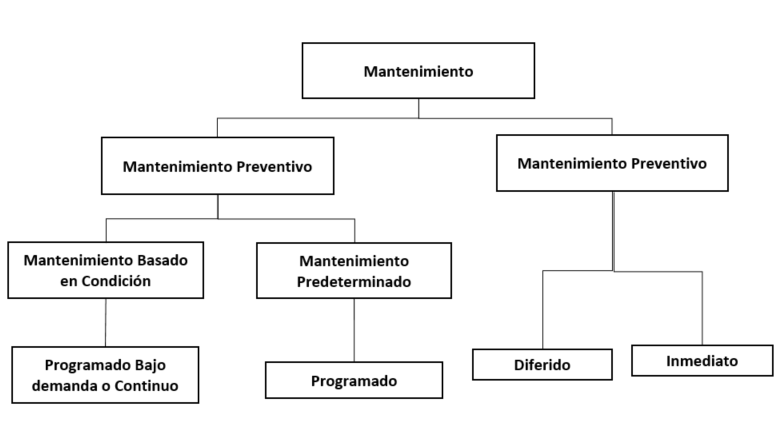
\includegraphics[width=3.9in]{Imagenes/TiposdeMtto} 

}

\caption{Clasificación general del mantenimiento según UNE-EN 13306. Fuente: UNE EN 13306}\label{fig:unnamed-chunk-1}
\end{figure}

\newpage

Por otra parte, la norma ISO -14224, que es una norma internacional que establece los principios y prácticas para la recopilación y el intercambio de datos de fiabilidad y mantenimiento para equipos industriales.
Esta norma proporciona un marco para la gestión de datos de fiabilidad con el objetivo de mejorar la gestión del ciclo de vida de los activos industriales.
Dividen en mantenimiento en categorías como:

\begin{itemize}
\item
  \begin{enumerate}
  \def\labelenumi{\alph{enumi})}
  \tightlist
  \item
    Aquellas que se realizan para corregir un ítem después de la falla (mantenimiento correctivo).
  \end{enumerate}
\item
  \begin{enumerate}
  \def\labelenumi{\alph{enumi})}
  \setcounter{enumi}{1}
  \tightlist
  \item
    Aquellas que se realizan para prevenir que un ítem caiga en estado de falla (mantenimiento preventivo); parte de esto pueden ser simplemente los chequeos (inspecciones, pruebas) para verificar la condición y el rendimiento del equipo con el fin de decidir si se requiere un mantenimiento preventivo.
  \end{enumerate}
\end{itemize}

Estas clasificaciones y categorías propuestas por esta norma se pueden evidenciar en la siguiente imagen.

\begin{figure}

{\centering 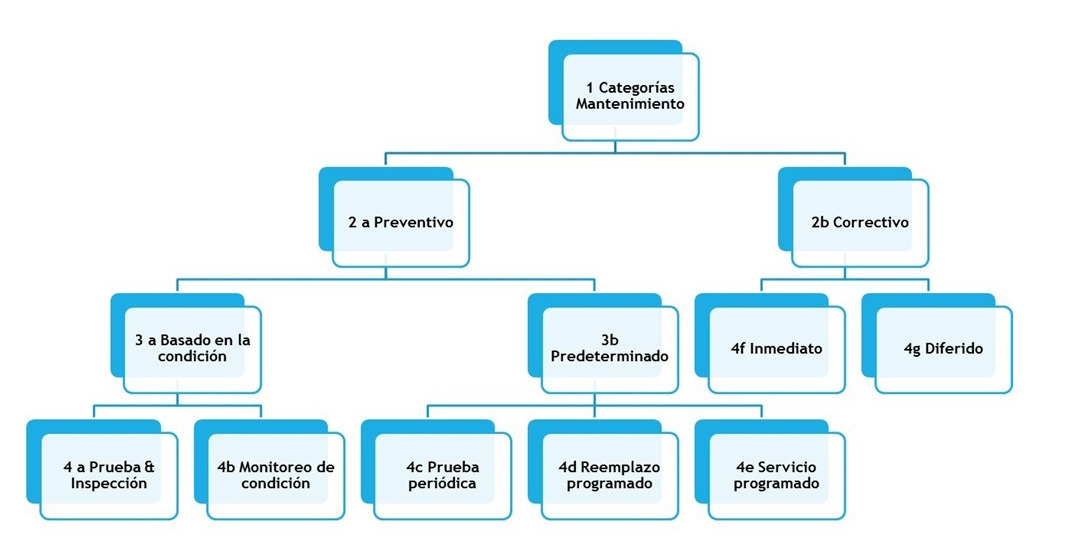
\includegraphics[width=5.37in]{Imagenes/categorias} 

}

\caption{Norma ISO 14224:2016}\label{fig:unnamed-chunk-2}
\end{figure}

Haciendo alusión a estos antecedentes históricos que han enmarcado el rumbo del mantenimiento industrial también existen otros puntos de vista interesantes de otros auntores como, \textcite{taylor1911principles} aborda la necesidad de aplicar métodos científicos al proceso de trabajo para mejorar la eficiencia y la productividad en las industrias.
Taylor propone un enfoque sistemático para analizar y estandarizar los procesos de trabajo, basado en la observación detallada y el estudio riguroso de cada tarea.

Una de las contribuciones clave de Taylor en su trabajo es el desarrollo del estudio de tiempos y movimientos.
Este método involucra la descomposición de las tareas en movimientos elementales y la determinación de los tiempos estándar para cada uno de ellos.
Al observar y medir repetidamente el tiempo necesario para realizar cada movimiento, los gerentes pueden establecer tiempos promedio y predecir con mayor precisión la duración total de una tarea.

En el contexto del mantenimiento industrial, Taylor argumenta que aplicar métodos científicos al estudio de los procesos de mantenimiento puede mejorar significativamente la eficiencia y la efectividad de las operaciones.
Al analizar en detalle cada paso del proceso de mantenimiento Haciendo alusión a estos antecedentes históricos que han enmarcado el rumbo del mantenimiento industrial también existen otros puntos de vista interesantes de otros auntores como, \textcite{taylor1911principles} aborda la necesidad de aplicar métodos científicos al proceso de trabajo para mejorar la eficiencia y la productividad en las industrias.
Taylor propone un enfoque sistemático para analizar y estandarizar los procesos de trabajo, basado en la observación detallada y el estudio riguroso de cada tarea.
Una de las contribuciones clave de Taylor en su trabajo es el desarrollo del estudio de tiempos y movimientos.
Este método involucra la descomposición de las tareas en movimientos elementales y la determinación de los tiempos estándar para cada uno de ellos.
Al observar y medir repetidamente el tiempo necesario para realizar cada movimiento, los gerentes pueden establecer tiempos promedio y predecir con mayor precisión la duración total de una tarea.
En el contexto del mantenimiento industrial, Taylor argumenta que aplicar métodos científicos al estudio de los procesos de mantenimiento puede mejorar significativamente la eficiencia y la efectividad de las operaciones.
Al analizar en detalle cada paso del proceso de mantenimiento y estandarizar los métodos de trabajo, las empresas pueden reducir los tiempos de inactividad y aumentar la disponibilidad de los equipos.

Como a porte al proyecto el enfoque de Taylor en los principios de la administración científica proporciona un sólido marco para elevar la eficiencia y efectividad de nuestras operaciones de mantenimiento industrial.

Este enfoque puede conducir a la reducción de costos, un aumento en la disponibilidad de equipos y una mejora en la competitividad de nuestra empresa.
Para alcanzar estos objetivos, estamos empleando técnicas de estadística multivariante como herramientas fundamentales en nuestro proceso de optimización.

\hypertarget{planes-de-mantenimiento-industrial.}{%
\subsubsection{Planes de mantenimiento Industrial.}\label{planes-de-mantenimiento-industrial.}}

Un plan de mantenimiento preventivo, según lo definido la norma ISO 14224, implica un enfoque sistemático y proactivo para mantener la disponibilidad y confiabilidad de los activos industriales.
Este tipo de plan se basa en la programación regular de inspecciones, ajustes, limpiezas, lubricaciones y reemplazos de componentes con el objetivo de prevenir fallas inesperadas.
Además, el plan incluye la recolección y el análisis de datos de fiabilidad y mantenimiento para mejorar continuamente las estrategias de mantenimiento y optimizar la vida útil de los equipos (ISO, 2016).
Estos planes de mantenimiento preventivo generalmente tienen una hoja de ruta donde se guardar las actividades a realizar, los materiales requeridos y el tiempo necesario para realizar la actividad y de acuerdo a dicha norma todo activo debe tener un plan de mantenimiento ya se preventivo, basado en condición o a falla.

Los planes de mantenimiento industrial son fundamentales en la gestión eficiente de activos en entornos productivos.
Estos planes no solo buscan corregir fallas una vez que ocurren, sino que también tienen como objetivo principal prevenir averías y maximizar la disponibilidad de la maquinaria y equipos industriales, Según \textcite{Martinez2020} La relevancia de los planes de mantenimiento industrial radica en su capacidad para mejorar la confiabilidad de los equipos y reducir los tiempos improductivos.
estos planes permiten realizar un seguimiento sistemático de las condiciones de los activos, anticipando posibles fallas y programando intervenciones preventivas.
En un entorno industrial, donde el tiempo de inactividad puede resultar costoso, contar con un plan de mantenimiento adecuado puede marcar la diferencia en términos de eficiencia y rentabilidad.

Gómez Poma, Jhon Angelo en su Artículo, Implementación de un plan de mantenimiento predictivo por análisis vibracional de la centrifugas continuas Broadbent y discontinuas Fives Cail de la empresa Cartavio S.A.A, menciona algunas pautas para implementar planes de mantenimientos y los problemas que causan las intervenciones no planificadas en el proceso productivo.
En términos generales proyecto exhibe los resultados alcanzables mediante la implemen- tación de un modelo predictivo para abordar problemas de fallas en máquinas.
Se observa que, tras la aplicación de esta técnica \textcite{gomez2022implementacion}, se logra mejorar la disponibilidad y aumentar la eficiencia del proceso productivo, al mejorar la eficiencia la maquina va a presentar menos fallos lo que indica menos tiempo en intervenciones correctivas.

\hypertarget{estaduxedstica-y-tiempos-de-mantenimiento-industrial}{%
\subsubsection{Estadística y tiempos de mantenimiento industrial}\label{estaduxedstica-y-tiempos-de-mantenimiento-industrial}}

\textcite{Assis2021} en su artículo ``A Dynamic Methodology for Setting Up Inspection Time Intervals in Conditional Preventive Maintenance'', manifiestan que uno de los principales problemas en el mantenimiento y especial el basado en condición es el de determinar los intervalos de tiempo de inspección y en proponen un método para determinar los tiempos requeridos utilizando técnicas estadísticas y en especial funciones de probabilidad como la distribución Weibull.
Para citar una aparte del resumen: ``Este artículo presenta un nuevo método para establecer un calendario óptimo para inspeccionar un componente crítico que falla debido al desgaste como lo describe una función de probabilidad de Weibull, Considerando un conjunto de intervalos de inspección, de modo que la confiabilidad entre cada dos inspecciones se mantenga igual o por debajo de un umbral preestablecido, manteniendo al mismo tiempo los costos totales de inspección, producción degradada, consecuencias de fallas y reparación al mínimo'' El anterior estudio es un gran aporte al proceso de mantenimiento, se evidencia como aplicando estas distribuciones se puede predecir la probabilidad que el equipo falle en un periodo de tiempo que también se traduce en la confiabilidad de la máquina, que pueda dar el rendimiento esperado en un periodo de tiempo sin presentar fallas.
Ellos hacen alusión a la distribución Weibull, de acuerdo a la literatura esta es ampliamente usada en la ingeniería como modelo para la descripción del tiempo de duración de un componente.
Esta distribución fue introducida por el científico sueco del mismo nombre, quien demostró que el esfuerzo al que se someten los materiales puede modelarse mediante el empleo de esta distribución.
\textcite{Castaneda2004}.
En el contexto de los Modelos Lineales Generalizados (GLM, por sus siglas en inglés), la distribución Weibull puede ser utilizada como una función de enlace para modelar variables de respuesta que no tienen una distribución normal.

Otra de las investigaciones realizadas donde se usa estadística para temas de mantenimiento, se describe en el artículo ``Preventive maintenance models -- higher operational reliability'' de los autores \textcite{Legat2017} Los autores presentan un método para determinar el intervalo óptimo para el mantenimiento periódico preventivo y un parámetro de diagnóstico óptimo para el mantenimiento/reemplazo predictivo.
Además, los autores plantean la pregunta: ¿cómo influye el mantenimiento preventivo en la probabilidad de falla y la confiabilidad operativa de los elementos del sistema que han sido sometidos a mantenimiento periódico preventivo?
Responden a la pregunta utilizando enfoques informáticos analíticos y de simulación.
Los resultados están en forma cuantitativa y dan relaciones entre los intervalos de mantenimiento preventivo y las funciones de confiabilidad.
Los ejemplos demuestran la idoneidad del método para objetos de ingeniería típicos que utilizan una distribución de Weibull de tres parámetros.
La aplicación del método supone un beneficio sustancial tanto para el fabricante como para el usuario del equipo técnico.

Revisando mas literatura \textcite{Nardo2021} en su artículo ``Development and implementation of an algorithm for preventive machine maintenance.Engineering Solid Mechanics,'' - Desarrollo e implementación de un algoritmo para el mantenimiento preventivo de máquinas

\begin{itemize}
\tightlist
\item
  \textbf{Resumen}: Este artículo tiene como objetivo desarrollar un modelo de optimización del mantenimiento para mantener un alto nivel de eficiencia y confiabilidad de la maquinaria. El enfoque metodológico se basa en el mantenimiento preventivo mediante la sustitución parcial o total de componentes críticos. Aunque se trata de un control de intervención intermedio, la atención se centra en una máquina concreta que se ha detenido varias veces, reduciendo su disponibilidad operativa y provocando un elevado coste de no producción. Este estudio utiliza un modelo de Weibull para analizar y optimizar el correcto proceso de mantenimiento de la maquinaria considerada. Luego, los datos de falla se analizan y programan. El objetivo final es estandarizar los procedimientos de intervención de los operadores para reducir el tiempo de las mismas intervenciones.
\end{itemize}

En el artículo anterior lo que buscan es encontrar el tiempo en el que una maquina presenta un fallo, con el fin de realizar la intervención antes de que se presente la avería y así no incurrir en costos por horas hombre correctivas, perdida de producción y repuestos no necesarios, proponen que se debe recopilar los datos históricos de mantenimiento y por medio de distribuciones y técnicas estadísticas tratar de predecir la confiabilidad y disponibilidad del equipo en periodo x de tiempo.

\hypertarget{impacto-del-mantenimiento-en-la-eficiencia-operativa}{%
\subsubsection{Impacto del mantenimiento en la eficiencia operativa}\label{impacto-del-mantenimiento-en-la-eficiencia-operativa}}

El mantenimiento en la industria desempeña un papel fundamental al asegurar que los equipos, maquinarias y sistemas funcionen de manera óptima, al funcionar bien la producción se mantiene y no se incurre en pérdidas lo menciona \textcite{Jardine2013}, el mantenimiento efectivo no solo se trata de reparar equipos cuando fallan y en los tiempos efectivos, lo importante de hacer mantenimiento es por medio de planes preventivos y predictivos prevenir averías o fallas antes de que ocurran, esta idea es respaldada por estudios como el de \textcite{Kumar2018}, quienes señalan que el mantenimiento preventivo puede reducir significativamente el tiempo de inactividad no planificado y mejorar la eficiencia de las operaciones industriales.

La importante de hacer mantenimiento y en especial el preventivo y predictivo es destacado por varios autores, para citar algunos.
\textcite{Olarte2010ImportanciaDM} Resalta la importancia de la planificación del mantenimiento para lograr altos niveles de calidad en cualquier tipo de empresa y proporciona una descripción histórica de los cambios en la implementación del modelo de mantenimiento en la industria, cuando se menciona planificación del mantenimiento se refiere al preventivo, que generalmente tiene un periodo de ejecución o frecuencia, un tiempo de ejecución y acciones a realizar, puntualizar que siempre el objetivo de este es conservar y prevenir que se presenten fallas.
\textcite{ARROYOVACA2022ImportanciaDL} subraya los beneficios del mantenimiento preventivo, incluido el aumento de la productividad, la reducción de los costos de mantenimiento y la prolongación de la vida útil de la maquinaria.

Para puntualizar de acuerdo a estos el mantenimiento industrial, con técnicas y planeación efectiva juega un papel crítico en la producción y la eficiencia operativa de las empresas industriales.
Es crucial que aplique enfoque integral que incluya estrategias preventivas, predictivas y correctivas puede minimizar el tiempo de inactividad, optimizar los recursos, mejorar la calidad del producto y aumentar la rentabilidad.
Estas consideraciones son fundamentales para que las empresas mantengan su competitividad en un entorno empresarial cada vez más dinámico y exigente.

\newpage

\hypertarget{estaduxedstica-y-modelos-de-predicciuxf3n}{%
\subsection{Estadística y Modelos de predicción}\label{estaduxedstica-y-modelos-de-predicciuxf3n}}

\hypertarget{estadistica-multivariada}{%
\subsubsection{Estadistica Multivariada}\label{estadistica-multivariada}}

``La estadística multivariada es una rama de la estadística que estudia la relación entre múltiples variables. Estos métodos permiten analizar la complejidad de los fenómenos reales, donde intervienen diversas variables que interactúan entre sí. Algunas de las técnicas multivariadas más empleadas son el análisis de componentes principales, el análisis factorial, el análisis discriminante y los modelos de ecuaciones estructurales. Estas herramientas son ampliamente utilizadas en campos como la economía, la psicología, la biología y la ingeniería para extraer información valiosa de conjuntos de datos multidimensionales'' \textcite{hair}.

``La estadística multivariada ha demostrado ser una herramienta poderosa en diversos campos de investigación. Por ejemplo, en el ámbito de la medicina, los métodos multivariados han sido utilizados para identificar factores de riesgo asociados a enfermedades, clasificar pacientes en grupos de tratamiento y modelar la progresión de dolencias crónicas. En el campo de las ciencias sociales, estas técnicas han permitido analizar la influencia de múltiples variables socioeconómicas en el comportamiento humano'' \textcite{Tabachnick2013}, para afirmar estos aportes y citando otros artículos anteriores donde varios autores experimentan con estás técnicas para predecir los tiempos efectivos para realizar un mantenimiento , caso de modelos de regresión y modelos de probabilidad como la distribución Weibull.

\hypertarget{tuxe9cnicas-de-estaduxedstica-multivariante.}{%
\subsubsection{Técnicas de estadística multivariante.}\label{tuxe9cnicas-de-estaduxedstica-multivariante.}}

Las técnicas de estadística multivariante son ideales para analizar conjuntos de datos que abarcan múltiples variables simultáneamente.
A diferencia de los modelos univariados, que se centran en una sola variable a la vez, estas técnicas exploran las complejas interrelaciones entre varias variables.
Esto permite una comprensión más profunda y completa de los datos.
El autor \textcite{anderson}, explica lo útiles que son para identificar interdependencias entre variables que podrían pasarse por alto en análisis univariados.
En la investigación moderna, donde las relaciones entre variables son la norma, esta capacidad para descubrir conexiones ocultas es fundamental.
Junto a Anderson el autor \textcite{hair} resalta los beneficios de estas técnicas, como la capacidad para capturar la complejidad inherente de conjuntos de datos multidimensionales que permite comprender mejor las relaciones subyacentes.
No obstante, a pesar de sus ventajas, las técnicas multivariadas presentan limitaciones importantes.
La interpretación de los resultados puede ser complicada, especialmente en la gestión de grandes conjuntos de datos con numerosas variables.
En situaciones donde la interpretación precisa es crucial, como en estudios médicos, esta complejidad puede representar un desafío significativo.
La asunción de linealidad también constituye una limitación relevante.
Aunque algunos métodos permiten extensiones no lineales, si las relaciones de las variables no son lineales los modelos podrían dar resultados no confiables al momento de predecir.
En nuestro contexto, donde buscamos predecir los tiempos de reparación de máquinas con fallos, la diversidad de técnicas disponibles nos proporciona la capacidad de modelar nuestra variable dependiente mediante múltiples técnicas buscando la que mejor se acople a la naturaleza de nuestros datos.

\hypertarget{modelo-de-regresiuxf3n-muxfaltiple}{%
\subsubsection{Modelo de regresión múltiple}\label{modelo-de-regresiuxf3n-muxfaltiple}}

El modelo de regresión lineal múltiple es una extensión del modelo de regresión lineal simple que permite explorar la relación entre una variable dependiente y múltiples variables independientes \textcite{montgomery2012introduction}.
En este modelo, la relación entre las variables se modela mediante un plano o un hiperplano en un espacio de varias dimensiones.
Los coeficientes de regresión representan el efecto de cada variable independiente en la variable dependiente \textcite{fox2015applied}.
Los modelos de regresión lineal múltiple son ampliamente utilizados en diversas áreas, como la economía, la sociología, la psicología y la epidemiología, entre otros \textcite{draper2014applied}.
Se utilizan para predecir o explicar el valor de una variable dependiente en función de múltiples variables independientes.

la fórmula general para un modelo de regresión lineal es la siguiente: \myequations{Modelo de regresión lineal}

\begin{equation}
\large Y = \beta_0 + \beta_1 X_1 + \beta_2 X_2 + \ldots + \beta_p X_p + \varepsilon\end{equation}

\begin{itemize}
\tightlist
\item
  \(Y\) es la variable dependiente que estamos tratando de predecir.
\item
  \(\beta_0\) es el intercepto o término constante.
\item
  \(\beta_1, \beta_2, \ldots, \beta_p\) son los coeficientes asociados con las variables predictoras \(X_1, X_2, \ldots, X_p\), respectivamente.
\item
  \(\varepsilon\) es el término de error, que representa la variabilidad no explicada por el modelo.
\end{itemize}

Los modelos de regresión lineal se basan en múltiples supuestos, como los siguientes:

\textbf{Linealidad}: Se asume que la relación entre las variables predictoras y la variable dependiente es lineal.
Esto implica que los cambios en las variables predictoras están asociados con cambios proporcionales en la variable de interés.

\textbf{Independencia de errores}: Se asume que los errores (residuos) de la regresión no están correlacionados entre sí.

\textbf{Homocedasticidad}: La varianza de los errores debe ser constante en todos los niveles de las variables predictoras.
Esto significa que la dispersión de los errores es uniforme en toda la gama de valores de las variables predictoras.

\textbf{Normalidad de errores}: Se asume que los errores de la regresión se distribuyen normalmente.
Esto significa que los residuos siguen una distribución normal con una media de cero.

\textbf{Independencia de variables predictoras}: Es crucial que las variables predictoras en un modelo de regresión sean independientes unas de otras.
Una elevada correlación entre estas variables puede entorpecer la interpretación precisa de los coeficientes, afectando la validez del modelo.

\hypertarget{modelos-lineales-generalizados-glm}{%
\subsubsection{Modelos Lineales Generalizados (GLM)}\label{modelos-lineales-generalizados-glm}}

Los Modelos Lineales Generalizados (GLM) constituyen una poderosa extensión de los modelos lineales tradicionales, permitiendo abordar una amplia gama de tipos de datos y distribuciones de error más allá de la normalidad.
A diferencia de los modelos lineales simples que asumen que la variable dependiente es normalmente distribuida, los GLM facilitan la modelización de la relación entre una variable dependiente, que puede seguir diversas distribuciones (como binomial, Poisson, o gamma), y una o más variables independientes a través de una función de enlace.

Esta capacidad para manejar diferentes distribuciones hace que los GLM sean particularmente adecuados para analizar datos donde la variable respuesta es, por ejemplo, una proporción, un conteo, o una medida de tiempo hasta un evento.
Esta versatilidad se discute ampliamente en la literatura, con \autocite{nelder1972generalized} siendo uno de los trabajos pioneros que estableció las bases teóricas de los GLM.

Los GLM son útiles en una variedad de campos, incluyendo la biometría, la epidemiología y las ciencias sociales, donde las variables de interés no se ajustan a la distribución normal.
Por ejemplo, en estudios de respuesta binaria como la presencia o ausencia de una enfermedad, los datos pueden modelarse efectivamente usando una distribución binomial con una función de enlace logit.

Una de las principales ventajas de los GLM es su capacidad para proporcionar estimaciones y pruebas inferenciales sobre los parámetros del modelo que son interpretables y útiles para la toma de decisiones.

Los GLM ofrecen un marco estadístico robusto y flexible para la modelización de relaciones entre variables, siendo capaces de abordar una amplia gama de situaciones de datos más allá de las limitaciones de los modelos lineales tradicionales.
Su aplicación en diversas áreas testimonia su valor en la investigación cuantitativa, como destaca \textcite{mccullagh1989generalized} en su obra sobre teoría y aplicaciones de los GLM.

La fórmula general de los GLM es la siguiente: \myequations{Modelo GLM}

\begin{equation}
\large g(\mu) = \beta_0 + \beta_1 \cdot x_1 + \beta_2 \cdot x_2 + \ldots + \beta_n \cdot x_n\end{equation}

\begin{itemize}
\item
  \(g(\mu)\): Representa la variable dependiente, es decir, la variable que estamos tratando de predecir.
  En el contexto de la regresión lineal, \(g(\mu)\) se estima como una combinación lineal de las variables independientes.
\item
  \(\beta_0\): Es el intercepto, también conocido como el coeficiente de intersección o término constante.
  Representa el valor esperado de la variable dependiente cuando todas las variables independientes son iguales a cero.
\item
  \(\beta_1, \beta_2, \ldots, \beta_n\): Son los coeficientes de regresión, que representan el cambio esperado en la variable dependiente debido a un cambio unitario en cada una de las variables independientes, manteniendo constantes todas las demás variables independientes.
\item
  \(x_1, x_2, \ldots, x_n\): Son las variables independientes o predictores.
  Cada una de estas variables puede tomar diferentes valores y se utilizan para predecir el valor de la variable dependiente \(g(\mu)\).
\end{itemize}

\hypertarget{modelo-de-regresiuxf3n-svr-support-vector-regression-svr}{%
\subsubsection{Modelo de regresión svr (Support Vector Regression, SVR)}\label{modelo-de-regresiuxf3n-svr-support-vector-regression-svr}}

La Regresión mediante Máquinas de Vectores de Soporte (SVR) emerge como una técnica innovadora en el ámbito del aprendizaje automático, evolucionando a partir de los principios establecidos por las Máquinas de Vectores de Soporte (SVM) para enfrentar desafíos específicos asociados con tareas de regresión.
Este enfoque se distingue por su capacidad para predecir valores continuos, aplicando un marco que equilibra la precisión predictiva con la complejidad del modelo para asegurar la generalización efectiva a datos no vistos.
El desarrollo conceptual y teórico de la SVR se apoya en la teoría de optimización y la teoría estadística del aprendizaje, particularmente en los trabajos de Vapnik y sus colaboradores, quienes han sido fundamentales en la formulación de las SVM y, por extensión, de la SVR \textcite{Vapnik1995}.

Central para la metodología de la SVR es la implementación de funciones kernel, que facilitan el mapeo no lineal de los datos de entrada a un espacio de alta dimensión donde las relaciones complejas entre variables pueden ser modeladas linealmente.
Esta característica es esencial para abordar con éxito datos que presentan patrones no lineales, permitiendo que la SVR se adapte a una amplia variedad de contextos y tipos de datos.
La selección del kernel adecuado (e.g., lineal, polinomial, RBF) y la calibración de sus parámetros son cruciales para el rendimiento del modelo, enfatizando la importancia de una comprensión detallada de la naturaleza del conjunto de datos y el problema específico a resolver \textcite{ScholkopfSmola2002}.

La formulación general de la Regresión mediante Máquinas de Vectores de Soporte (SVR) busca encontrar una función \(f(x)\) que tenga a lo más un \(\epsilon\)-desvío de los valores reales \(y_i\) para todas las muestras de entrenamiento, y al mismo tiempo sea lo más plana posible.
Matemáticamente, esto se traduce en minimizar la siguiente función objetivo:

\myequations{Función objetivo de la Regresión SVR}

\begin{equation}
\large \min_{w, b, \xi, \xi^*} \frac{1}{2} \|w\|^2 + C \sum_{i=1}^{n} (\xi_i + \xi_i^*) \end{equation}

Sujeto a las restricciones:

\[
\begin{aligned}
y_i - \langle w, x_i \rangle - b &\leq \epsilon + \xi_i, \\
\langle w, x_i \rangle + b - y_i &\leq \epsilon + \xi_i^*, \\
\xi_i, \xi_i^* &\geq 0, &\text{ para todo } i = 1, \ldots, n.
\end{aligned}
\]

Donde:

\begin{itemize}
\item
  \(x_i\) son las características de entrada
\item
  \(y_i\) son los valores objetivo
\item
  \(w\) es el vector de pesos
\item
  \(b\) es el término de sesgo
\item
  \(\xi_i\) y \(\xi_i^*\) son variables de holgura que miden el grado de desviación permitido para errores por encima y por debajo de \(\epsilon\), respectivamente
\item
  \(C\) es el parámetro de regularización que establece el balance entre la suavidad de la función \(f(x)\) y el grado hasta el cual desviaciones mayores que \(\epsilon\) son toleradas.
\end{itemize}

\hypertarget{modelo-de-regresiuxf3n-con-uxe1rboles-de-decisiuxf3n}{%
\subsubsection{Modelo de Regresión con Árboles de Decisión}\label{modelo-de-regresiuxf3n-con-uxe1rboles-de-decisiuxf3n}}

La Regresión mediante Árboles de Decisión representa una metodología destacada en el dominio del aprendizaje supervisado, extendiendo los principios fundamentales de los árboles de decisión hacia la predicción de valores continuos.
Este enfoque se caracteriza por su habilidad para manejar de manera intuitiva tanto relaciones lineales como no lineales entre las variables, mediante la división del espacio de características en regiones homogéneas.
El desarrollo de los árboles de decisión para regresión se nutre de conceptos sólidos de teoría de la información y estadísticas, apoyándose en criterios de división como la reducción de la varianza y el error cuadrático medio para optimizar las decisiones de partición \textcite{Breiman1984}.

Un aspecto crucial de los árboles de decisión en la regresión es su capacidad para adaptarse automáticamente a las complejidades de los datos, permitiendo una modelización flexible de interacciones entre variables sin requerir especificaciones de modelo predefinidas.
La estructura del árbol de decisión, compuesta por nodos de decisión y hojas, ofrece una representación gráfica que facilita la interpretación de cómo las características influyen en la predicción final.
La selección de parámetros como la profundidad máxima del árbol y el mínimo número de muestras requeridas para un nodo, juegan un papel esencial en prevenir el sobreajuste y asegurar una buena generalización del modelo \textcite{Quinlan1993}.

La formulación general de la regresión con árboles de decisión busca construir un modelo que particione el espacio de características de manera que las predicciones en cada región sean lo más precisas posible, minimizando una función de pérdida predeterminada, típicamente el error cuadrático.
Esta meta se consigue mediante la siguiente representación general:

\myequations{Función objetivo de la Regresión con Árboles de Decisión}

\begin{equation}
\large \min_{\theta} \sum_{i=1}^{n} L(y_i, f(x_i;\theta)),
\end{equation}

donde:

\begin{itemize}
\tightlist
\item
  \(x_i\) son las características de entrada
\item
  \(y_i\) son los valores objetivo
\item
  \(\theta\) representa los parámetros del modelo, incluyendo las decisiones de división y las predicciones en cada hoja
\item
  \(L\) es la función de pérdida, usualmente el error cuadrático medio entre las predicciones y los valores reales.
\end{itemize}

La construcción de un árbol de decisión implica seleccionar las divisiones que más reduzcan la función de pérdida en el conjunto de datos de entrenamiento, con un proceso iterativo de partición binaria.
Las técnicas de poda y validación cruzada se emplean frecuentemente para afinar el modelo y evitar el sobreajuste, manteniendo un equilibrio entre la complejidad del modelo y su capacidad predictiva.

\hypertarget{modelo-de-regresiuxf3n-con-random-forest}{%
\subsubsection{Modelo de Regresión con Random Forest}\label{modelo-de-regresiuxf3n-con-random-forest}}

La regresión con Random Forest es una técnica robusta de aprendizaje automático que construye y combina múltiples árboles de decisión para mejorar la precisión y la capacidad de generalización de las predicciones.
A diferencia de un solo árbol de decisión, Random Forest incorpora la sabiduría de la multitud mediante la agregación de los resultados de numerosos árboles para formar la predicción final, un proceso conocido como ``bagging'' o ``Bootstrap Aggregating'' \textcite{breiman2001random} .

Esta técnica sobresale en su capacidad de manejar grandes conjuntos de datos con múltiples variables de entrada, siendo capaz de capturar interacciones complejas y no lineales sin necesidad de una especificación de modelo detallada.
Random Forest es particularmente conocido por su robustez ante el sobreajuste, gracias a la aleatoriedad introducida durante la construcción de los árboles, que incluye la selección de características y muestras.

Al igual que con los árboles individuales, la regresión con Random Forest opera dividiendo el espacio de las características en subespacios, pero mejora la estabilidad y precisión al promediar múltiples árboles, reduciendo la varianza sin aumentar el sesgo.

El desarrollo de un modelo de Random Forest para regresión sigue principios estadísticos sólidos, empleando el promedio de las predicciones de los árboles individuales para minimizar el error total y proporcionar una estimación más fiable y precisa.
En el corazón de Random Forest, la diversidad entre los árboles se fomenta a través de dos mecanismos principales:

Bootstrap de muestras: Cada árbol se entrena con una muestra aleatoria del conjunto de datos (con reemplazo), permitiendo que diferentes árboles aprendan de distintas porciones de los datos.
Selección aleatoria de características: En cada división, se selecciona un subconjunto aleatorio de las características disponibles, lo que obliga a los árboles a tomar decisiones basadas en diferentes combinaciones de entradas.
Estos procesos se resumen en la siguiente fórmula general de Random Forest para regresión:

\myequations{Función objetivo de la Regresión con Random Forest}

\begin{equation}
\large \min_{\{\theta_k\}} \frac{1}{K} \sum_{k=1}^{K} \sum_{i \in B_k} L(y_i, f(x_i;\theta_k)),
\end{equation}

donde:

\begin{itemize}
\tightlist
\item
  \(K\) es el número de árboles en el bosque.
\item
  \(B_k\) es el conjunto de datos bootstrap para el k-ésimo árbol.
\item
  \(f(x_i;\theta_k)\) es la predicción del k-ésimo árbol con parámetros \(\theta_k\).
\item
  \(L\) es la función de pérdida, que continúa siendo comúnmente el error cuadrático medio.
\end{itemize}

Los parámetros importantes de un Random Forest incluyen el número de árboles (ntree), el número de variables consideradas para dividir en cada nodo (mtry), y el tamaño mínimo de los nodos de hoja.
La selección de estos hiperparámetros se realiza típicamente mediante técnicas de búsqueda como la validación cruzada y la búsqueda en cuadrícula o aleatoria.

La interpretación de un modelo de Random Forest puede ser menos directa en comparación con un único árbol de decisión debido a la naturaleza agregada de la predicción.
No obstante, los métodos de importancia de las variables proporcionan perspectivas significativas sobre la contribución de cada característica al modelo, ayudando a identificar los predictores más relevantes.

\hypertarget{otros-modelos-de-regresiuxf3n}{%
\subsubsection{Otros modelos de regresión}\label{otros-modelos-de-regresiuxf3n}}

Los modelos mencionados a continuación también son capaces de predecir el valor de una variable dependiente a partir de varias variables independientes.
No obstante, una limitación significativa de estos en comparación con los modelos previamente discutidos es su incapacidad para ofrecer de manera directa una evaluación sobre el impacto o la relevancia de cada variable independiente en el resultado de la predicción.
Esta carencia obstaculiza la comprensión detallada de la contribución específica de cada variable al resultado final, lo cual es esencial para una interpretación profunda y la toma de decisiones informadas basadas en el modelo.

\hypertarget{modelos-lineales-mixtos-lmm}{%
\paragraph{Modelos Lineales Mixtos (LMM)}\label{modelos-lineales-mixtos-lmm}}

Los Modelos Lineales Mixtos (LMM) son una clase de modelos estadísticos utilizados para el análisis de datos en los que las observaciones no son independientes entre sí, como es común en datos longitudinales o de panel \textcite{pinheiro2000mixed}.
Los LMM combinan elementos de los Modelos Lineales Generalizados (GLM) con la capacidad de manejar la estructura de dependencia entre las observaciones.

En un LMM, se asume que los datos tienen una estructura jerárquica, donde las observaciones están agrupadas en unidades o clústeres, como en nuestro caso las diferentes disciplinas encargadas de las reparaciones.
La inclusión de efectos aleatorios en el modelo permite capturar la variabilidad entre estos grupos, lo que mejora la precisión de las estimaciones y la capacidad de generalización del modelo \textcite{gelman2006data}.

Los LMM se pueden utilizar para modelar tanto respuestas continuas como categóricas, y pueden incluir tanto efectos fijos como efectos aleatorios.
Los \textbf{efectos fijos} representan las relaciones promedio entre las variables independientes y la variable dependiente, mientras que los \textbf{efectos aleatorios} capturan la variabilidad entre los grupos o clústeres \textcite{gelman2006data}.

Algunas aplicaciones comunes de los LMM incluyen estudios longitudinales, para analizar datos recogidos a lo largo del tiempo, estudios multinivel, para analizar datos estructurados en múltiples niveles jerárquicos, y estudios espaciales, para analizar datos recogidos en ubicaciones geográficas diferentes \textcite{gelman2006data}.

Los LMM se pueden ajustar utilizando diferentes métodos de estimación, como la máxima verosimilitud restringida (REML) o la estimación de la máxima verosimilitud (MLE).
Para trabajar con este modelo en R podemos utilizar paquetes como lme4 creado por \textcite{bates2015lme4} siendo este paquete útil para ajustar y analizar modelos lineales mixtos de manera eficiente y efectiva.

La fórmula general de un modelo LMM es la siguiente:

\myequations{Modelo LMM}

\begin{equation}
\large y_{ij} = \beta_0 + \beta_1 \cdot x_{ij} + u_{j} + \varepsilon_{ij}\end{equation}

\begin{itemize}
\item
  \(y_{ij}\): Representa la variable dependiente en la observación \(i\) del grupo \(j\).
\item
  \(\beta_0\): Es el intercepto, que representa el valor esperado de la variable dependiente cuando todas las variables explicativas son cero.
\item
  \(\beta_1\): Es el coeficiente de regresión, que indica el cambio esperado en la variable dependiente \(y_{ij}\) por cada unidad de cambio en la variable explicativa \(x_{ij}\).
\item
  \(x_{ij}\): Representa la variable explicativa en la observación \(i\) del grupo \(j\).
\item
  \(u_j\): Son los efectos fijos, que capturan las características específicas del grupo \(j\) que no varían dentro de ese grupo pero pueden variar entre grupos.
\item
  \(\varepsilon_{ij}\): Es el término de error, que representa el error aleatorio en la predicción del modelo.
\end{itemize}

\hypertarget{modelos-lineales-generalizados-mixtos-glmm}{%
\paragraph{Modelos Lineales Generalizados Mixtos (GLMM)}\label{modelos-lineales-generalizados-mixtos-glmm}}

Los Modelos Lineales Generalizados Mixtos (GLMM) son una extensión de los Modelos Lineales Generalizados (GLM) que permiten modelar la relación entre variables predictoras y una variable respuesta, teniendo en cuenta la estructura de dependencia entre las observaciones y la inclusión de efectos aleatorios.

Estos modelos resultan especialmente valiosos cuando los datos presentan una estructura jerárquica o correlacionada, como sucede en casos de datos longitudinales, de panel o agrupados, como en nuestra situación donde podemos agrupar los datos por disciplina.
La principal ventaja de los GLMM frente a modelos lineales y LMM radica en su capacidad para manejar datos no normales y aun así analizar sus efectos fijos, tal como aborda el autor \textcite{bolker2009generalized} en su análisis sobre ecología y evolución.

Además, los GLMM ofrecen una mayor flexibilidad para modelar diferentes tipos de variables respuesta y estructuras de datos, así como una mejor capacidad para capturar la variabilidad entre grupos.
Asimismo, permiten interpretar la varianza residual y descomponerla en componentes atribuibles a los efectos fijos y aleatorios, lo que facilita la interpretación de la variabilidad observada en los datos.

Para concluir los GLMM representan una herramienta estadística poderosa y flexible para modelar relaciones entre variables predictoras y una variable respuesta en presencia de estructuras de datos jerárquicas o correlacionadas, y son especialmente útiles en campos como la ecología, la biología, la epidemiología y las ciencias sociales \textcite{zuur2009mixed}.

La fórmula general de los glmm es la siguiente: \myequations{Modelo GLMM}

\begin{equation}
\large g(\mu_{ij}) = \beta_0 + \beta_1 \cdot x_{ij} + u_{j}\end{equation}

\hypertarget{maching-learning}{%
\subsection{Maching Learning}\label{maching-learning}}

El machine Learning o aprendizaje automático, es un subcampo de las ciencias de computación que tienen como finalidad establecer algoritmos para que las computadoras aprendan patrones de datos a gran escala con el fin de extraer información que mejoren los procesos de análisis de los datos, el Machine Learning (ML) se ha consolidado como una herramienta fundamental para extraer conocimiento y generar predicciones acertadas.
El Machine Learning, definido por Arthur Samuel en 1959 como ``el campo de estudio que da a las computadoras la habilidad de aprender sin ser explícitamente programadas'' \textcite{Samuel1959}, ha evolucionado rápidamente en las últimas décadas, convirtiéndose en un pilar clave para la toma de decisiones informadas en una amplia gama de industrias y campos de investigación.

A diferencia de los enfoques de programación tradicionales, donde los algoritmos se basan en instrucciones y reglas definidas explícitamente, el Machine Learning permite que los sistemas aprendan y mejoren automáticamente a partir de los datos.
Esto se logra a través de la aplicación de técnicas como el aprendizaje supervisado, el aprendizaje no supervisado y el aprendizaje por refuerzo, cada uno de los cuales aborda diferentes tipos de problemas y desafíos \textcite{Hastie2009}.

\hypertarget{aprendizaje-supervisado}{%
\paragraph{Aprendizaje Supervisado}\label{aprendizaje-supervisado}}

El aprendizaje supervisado se conoce por su capacidad de extraer conocimiento a partir de datos etiquetados, permitiendo a los algoritmos establecer relaciones entre variables de entrada y variables de salida para generar predicciones y clasificaciones precisas.

En el aprendizaje supervisado, el algoritmo tiene acceso a un conjunto de datos de entrenamiento que contiene observaciones o instancias con valores conocidos para la variable de salida.
Esto le permite al modelo ``aprender'' a reconocer patrones y construir una función que mapee adecuadamente las entradas a las salidas deseadas \textcite{Hastie2009}, Por citar un ejemplo, en mantenimiento un problema de predicción de tiempos , el algoritmo utilizaría datos históricos de tiempos correctivos, con información sobre variables como total horas, estado del equipo, frecuencia de mantenimientos y tiempos empleados para reparaciones anteriores, para establecer un modelo que permita pronosticar los tiempos a futuro.

Dentro del aprendizaje supervisado, existen dos tipos principales de problemas: regresión y clasificación.
Los problemas de regresión buscan predecir una variable numérica continua, como el precio de una acción o la demanda de un producto.
Por otro lado, los problemas de clasificación tienen como objetivo asignar instancias a categorías o clases discretas, como determinar si un correo electrónico es spam o no spam \textcite{Witten2016}.
Este se consolida como una herramienta fundamental en el campo del Machine Learning, permitiendo a los investigadores y profesionales generar predicciones y clasificaciones precisas a partir de datos etiquetados.
A medida que la disponibilidad y complejidad de los datos continúan aumentando, el aprendizaje supervisado seguirá desempeñando un papel crucial en la toma de decisiones informadas en diversos ámbitos

\hypertarget{aprendizaje-no-supervisado}{%
\paragraph{Aprendizaje No Supervisado}\label{aprendizaje-no-supervisado}}

A diferencia del aprendizaje supervisado, el aprendizaje no supervisado es una rama crucial del machine learning que se enfoca en descubrir patrones y estructuras ocultas en conjuntos de datos sin etiquetar, Según \textcite{Bishop2006}, el aprendizaje no supervisado implica encontrar una representación útil o una estructura subyacente en los datos sin conocer las salidas esperadas.
Esto es especialmente útil en situaciones donde los datos pueden no estar etiquetados o cuando se desea explorar la naturaleza intrínseca de los datos sin ninguna suposición previa sobre las relaciones entre variables.

Algunos de los principales métodos de aprendizaje no supervisado incluyen el análisis de conglomerados (clustering), la reducción de dimensionalidad y la detección de anomalías \textcite{Witten2016}.
El análisis de conglomerados tiene como finalidad agrupar las observaciones en función de sus características, de manera que los elementos dentro de un mismo grupo sean similares entre sí y diferentes a los de otros grupos.
Esto resulta útil para segmentación de clientes, identificación de tipos de consumidores, o agrupación de genes con funciones biológicas similares.

Resaltar que una de las principales fortalezas del aprendizaje no supervisado es su capacidad de descubrir patrones y relaciones inesperadas en los datos, lo que puede conducir a nuevos conocimientos y oportunidades de innovación.
Además, estas técnicas son especialmente útiles cuando los datos disponibles no cuentan con etiquetas o variables de salida claras, como en el análisis exploratorio de conjuntos de datos complejos.
Para citar algunos algoritmos de aprendizaje No Supervisado: K-Means, DBSCAN, Algoritmos de Agrupamiento Jerárquico, Análisis de Componentes Principales (PCA), t-distributed Stochastic Neighbor Embedding, Gaussian Mixture Models (GMM), Isolation Forest.

\hypertarget{conceptos-y-definiciones}{%
\subsection{Conceptos y definiciones}\label{conceptos-y-definiciones}}

\hypertarget{r-studio}{%
\subsubsection{R Studio}\label{r-studio}}

R destaca por su notable flexibilidad, permitiendo la aplicación de una amplia gama de modelos estadísticos y matemáticos.
Desde simples modelos lineales hasta técnicas avanzadas como regresión logística, árboles de decisión, redes neuronales y análisis de series temporales, R ofrece una completa variedad de herramientas para el modelado predictivo y descriptivo.

Una de las principales fortalezas de R reside en su extensa colección de paquetes especializados, los cuales abarcan una amplia diversidad de áreas, desde el análisis estadístico más básico hasta técnicas de modelado más sofisticadas.
Estos paquetes son desarrollados y mantenidos tanto por la comunidad de usuarios como por expertos en diversos campos, asegurando una amplia disponibilidad de herramientas para abordar cualquier tarea de modelado que se presente.

\textbf{Paquetes necesarios}

\begin{itemize}
\item
  \textbf{DT:} \texttt{DT} proporciona una interfaz R para las DataTables de JavaScript, permitiendo la creación de tablas HTML interactivas que pueden ser visualizadas en R Markdown y aplicaciones Shiny.
  Este paquete es especialmente útil para la presentación de datos de forma dinámica, donde el usuario puede ordenar, filtrar y paginar la información directamente desde la visualización generada.
\item
  \textbf{lmtest:} El paquete \texttt{lmtest} ofrece una amplia gama de pruebas estadísticas para la evaluación de modelos lineales en R.
  Incluye herramientas para realizar pruebas de coeficientes, comparaciones de modelos, diagnósticos de residuos, entre otros.
  \texttt{lmtest} es valioso para analistas y estadísticos que buscan validar y comparar modelos lineales mediante pruebas rigurosas y basadas en criterios estadísticos sólidos.
\item
  \textbf{car:} \texttt{car} (Companion to Applied Regression) está diseñado para complementar el análisis de regresión aplicada en R, proporcionando una serie de funciones y conjuntos de datos útiles para el diagnóstico y la visualización de modelos lineales.
  Desde análisis de varianza hasta gráficos de influencia y diagnóstico, \texttt{car} facilita una comprensión más profunda de los modelos lineales y sus supuestos.
\item
  \textbf{lme4:} \texttt{lme4} se utiliza para ajustar modelos lineales mixtos y modelos lineales generalizados mixtos en R, ofreciendo una solución robusta para el análisis de datos con estructuras de dependencia complejas o agrupadas.
  Es ideal para datos jerárquicos, longitudinales o de panel, permitiendo a los investigadores modelar efectos tanto fijos como aleatorios y entender la variabilidad en los datos a múltiples niveles.
\item
  \textbf{lubridate:} \texttt{lubridate} simplifica el manejo de fechas y horas en R, proporcionando funciones intuitivas para la manipulación, el parseo y el cálculo con objetos de tiempo.
  Este paquete resuelve muchos de los desafíos comunes al trabajar con datos temporales, facilitando la conversión entre formatos de fecha y hora, la gestión de zonas horarias, y la realización de operaciones aritméticas con fechas.
\item
  \textbf{MuMIn:} \texttt{MuMIn} es un paquete en R dedicado a la selección y promedio de modelos, basado en criterios de información como el AIC o BIC.
  Resulta especialmente útil en la comparación exhaustiva de modelos candidatos y en la síntesis de los resultados a través del promedio de modelos, proporcionando así una visión más holística de los efectos modelados y ayudando a mejorar la precisión predictiva.
\item
  \textbf{ggthemes:} \texttt{ggthemes} extiende las capacidades de \texttt{ggplot2} al ofrecer una variedad de temas y escalas adicionales para la personalización de gráficos en R.
  Desde estilos inspirados en medios de comunicación y software famosos hasta paletas de colores adaptadas para una visualización de datos más atractiva y profesional, \texttt{ggthemes} enriquece la presentación visual de los análisis.
\item
  \textbf{rpart:} El paquete \texttt{rpart} facilita la implementación de árboles de decisión para clasificación y regresión en R.
  Utilizando el enfoque CART (Árboles de Clasificación y Regresión), \texttt{rpart} permite a los usuarios explorar la estructura de los datos y hacer predicciones basadas en las relaciones identificadas entre las variables.
  Es ampliamente utilizado tanto en análisis exploratorios como en la construcción de modelos predictivos complejos.
\item
  \textbf{e1071:} \texttt{e1071} trae a R una serie de algoritmos de aprendizaje automático y estadística, incluyendo máquinas de vectores de soporte (SVM), clasificación Naive Bayes, y análisis de componentes principales (PCA).
  Desarrollado inicialmente en la Universidad Tecnológica de Viena, este paquete es una herramienta esencial para tareas de clasificación, regresión y reducción de dimensionalidad en análisis de datos avanzados.
\end{itemize}

\hypertarget{pyhton}{%
\subsubsection{Pyhton}\label{pyhton}}

Python es un lenguaje de programación de alto nivel, interpretado y de propósito general.
Es conocido por su sintaxis clara y legible, lo que lo hace ideal para principiantes y programadores experimentados por igual.
Python es ampliamente utilizado en una variedad de campos, incluyendo desarrollo web, ciencia de datos, inteligencia artificial, automatización de tareas, entre otros.
Se destaca por su amplia biblioteca estándar y su comunidad activa que contribuye con paquetes y recursos para facilitar el desarrollo de software.
\textcite{PythonSoftwareFoundation2022}

\textbf{Paquetes y librerías utilizadas}

• Sckit-Learn: Scikit-Learn es una biblioteca de aprendizaje automático de código abierto para el lenguaje de programación Python.
Proporciona una amplia gama de algoritmos de aprendizaje supervisado y no supervisado, así como herramientas para la preparación, evaluación y visualización de datos.
Scikit-Learn es ampliamente utilizado en la comunidad de ciencia de datos y machine learning debido a su facilidad de uso, su documentación detallada y su integración con otras bibliotecas populares de Python, como NumPy, Pandas y Matplotlib

• NumPy: abreviatura de ``Numerical Python'', es una biblioteca de código abierto para el lenguaje de programación Python.
Proporciona soporte para arrays y matrices multidimensionales, junto con una amplia colección de funciones matemáticas de alto nivel para operar en estas estructuras de datos.
NumPy es fundamental en el ecosistema de Python para computación científica y análisis de datos, ya que ofrece una eficiente manipulación de datos numéricos, cálculos numéricos rápidos y funciones para trabajar con arrays de manera eficiente.

• Pandas: es una poderosa biblioteca de código abierto para el lenguaje de programación Python, diseñada principalmente para el análisis y manipulación de datos.
Proporciona estructuras de datos flexibles y eficientes, como DataFrames y Series, que permiten a los usuarios trabajar con datos tabulares de una manera intuitiva y eficaz.
Pandas es ampliamente utilizado en la comunidad de ciencia de datos y análisis de datos para tareas como limpieza, manipulación, exploración y análisis de datos.
\textcite{McKinney2010}.

• Matplotlib: es una biblioteca de visualización de datos de código abierto para el lenguaje de programación Python.
Proporciona una amplia variedad de herramientas para crear gráficos estáticos, interactivos y animados de manera sencilla y flexible.
Matplotlib es ampliamente utilizado en la comunidad de ciencia de datos, análisis de datos, investigación científica y educación debido a su versatilidad y capacidad para producir gráficos de alta calidad en diversos formatos y estilos \textcite{Hunter2007}.

\hypertarget{variables-y-tipos-de-variables}{%
\subsubsection{Variables y Tipos de Variables}\label{variables-y-tipos-de-variables}}

En el ámbito de la investigación, el concepto de variables es fundamental para comprender y analizar datos.
Las variables son características, propiedades o rasgos que pueden medirse, observarse o manipularse en un estudio.
Son elementos clave que los investigadores estudian y comparan para entender las relaciones entre ellos y cómo influyen en un fenómeno o proceso.
Una variable es cualquier cantidad que pueda tener más de un valor.
En un estudio científico, las variables son las características o atributos que se miden para evaluar los efectos de las condiciones experimentales.
Estas pueden ser tan simples como la edad de una persona o tan complejas como el nivel de contaminación en un área determinada.

Las variables se dividen en dos categorías:

\textbf{a. Variables Independientes:} Estas son las variables que un investigador manipula o cambia para observar su efecto sobre otras variables.
En un experimento, la variable independiente es la que se controla deliberadamente para ver cómo afecta a la variable dependiente.
Por ejemplo, en un estudio sobre el efecto de la luz en el crecimiento de las plantas, la cantidad de luz sería la variable independiente.

\textbf{a. Variables Dependientes:} Son las variables que se observan y miden en respuesta a los cambios en la variable independiente.
En el ejemplo de las plantas, el crecimiento de las plantas sería la variable dependiente, ya que se espera que cambie en respuesta a la cantidad de luz que reciben.

\hypertarget{tipos-de-variables}{%
\paragraph{Tipos de Variables}\label{tipos-de-variables}}

Las variables pueden clasificarse aún más en diferentes tipos, lo que ayuda a los investigadores a comprender mejor cómo analizar y presentar los datos.
Algunas de las clasificaciones comunes son:

\textbf{a. Variables Categóricas o Nominales:} Estas variables representan categorías discretas que no tienen un orden inherente.
Ejemplos incluyen el género, el estado civil, el tipo de vehículo (automóvil, camión, motocicleta), etc.
Se pueden codificar como números, pero estos números no tienen un significado numérico intrínseco.

\textbf{b. Variables Ordinales:} Las variables ordinales tienen categorías con un orden específico, pero las diferencias entre las categorías no son necesariamente iguales.
Por ejemplo, una escala de ``satisfacción'' que va desde ``muy insatisfecho'' hasta ``muy satisfecho'' es una variable ordinal.

\textbf{c.~Variables de Intervalo:} Estas variables tienen un orden significativo entre los valores y las diferencias entre los valores son igualmente significativas.
Sin embargo, no hay un punto cero absoluto.
Un ejemplo común es la temperatura en grados Celsius o Fahrenheit.
En la escala Celsius, por ejemplo, la diferencia entre 20°C y 30°C es la misma que entre 30°C y 40°C.

\textbf{d.~Variables de Razón:} Son similares a las variables de intervalo, pero tienen un cero absoluto, lo que significa que el valor cero representa la ausencia completa de la característica que se está midiendo.
Por ejemplo, la altura, el peso, el tiempo y la cantidad de dinero son variables de razón.
No tener dinero (0) es diferente de tener \$10 o \$20.

\hypertarget{pruebas-de-bondad-y-ajuste}{%
\subsubsection{Pruebas de bondad y ajuste}\label{pruebas-de-bondad-y-ajuste}}

Las pruebas de bondad de ajuste e independencia son ampliamente utilizadas en diversas áreas de la ciencia para llevar a cabo análisis de datos.
Una prueba de bondad de ajuste permite evaluar la hipótesis de que una variable aleatoria sigue cierta distribución de probabilidad y se utiliza en situaciones donde se requiere comparar una distribución observada con una teórica o hipotética, compararla con datos históricos o con la distribución conocida de otra población.

Las pruebas más utilizadas para estudiar la independencia y la bondad de ajuste son las chicuadrado de Pearson, el estadístico de Kolmogorov-Smirnov, criterio de información de Akaike (AIC) entre otros debido a su fácil aplicación y a que se encuentran en todos los paquetes estadísticos.
Estas pruebas asumen que todas las observaciones son independientes y que están igualmente distribuidas, supuestos que sólo se satisfacen para un muestreo aleatorio simple con reposición y se cumplen aproximadamente en una muestra aleatoria simple sin reposición para una fracción de muestreo pequeña \textcite{QuinteroM2014}.

\hypertarget{distribuciuxf3n-de-probabilidad.}{%
\subsubsection{Distribución de probabilidad.}\label{distribuciuxf3n-de-probabilidad.}}

En teoría de la probabilidad y estadística, la distribución de probabilidad de una variable aleatoria es una función que asigna a cada suceso definido sobre la variable la probabilidad de que dicho suceso ocurra.
La distribución de probabilidad está definida sobre el conjunto de todos los sucesos y cada uno de los sucesos es el rango de valores de la variable aleatoria.
También puede decirse que tiene una relación estrecha con las distribuciones de frecuencia.
De hecho, una distribución de probabilidades puede comprenderse como una frecuencia teórica, ya que describe cómo se espera que varíen los resultados.

La distribución de probabilidad está completamente especificada por la función de distribución, cuyo valor en cada x real es la probabilidad de que la variable aleatoria sea menor o igual que x.

\hypertarget{modelos-en-mantenimiento-industrial}{%
\subsubsection{Modelos en mantenimiento Industrial:}\label{modelos-en-mantenimiento-industrial}}

En el contexto del mantenimiento industrial, la aplicación de modelos multivariables y de series temporales juega un papel fundamental en la predicción del tiempo necesario para reparar máquinas en un intervalo específico.
Estos modelos contribuyen significativamente a la eficiencia y fiabilidad de los procesos industriales.

\hypertarget{optimizaciuxf3n-de-procesos}{%
\subsubsection{Optimización de Procesos:}\label{optimizaciuxf3n-de-procesos}}

La optimización de tiempos de atención de fallas en redes eléctricas y en el mantenimiento industrial se enfoca en reducir los tiempos de respuesta ante situaciones de emergencia, garantizando la seguridad del personal y la eficacia en la asignación de recursos.

\hypertarget{limitaciones-y-consideraciones}{%
\subsubsection{Limitaciones y Consideraciones:}\label{limitaciones-y-consideraciones}}

A pesar de las ventajas de las técnicas de estadística multivariante, como la capacidad para identificar interdependencias entre variables, es importante considerar las limitaciones en la interpretación de resultados, especialmente en conjuntos de datos complejos.
La asunción de linealidad también puede ser un desafío en ciertos contextos.

\hypertarget{distribuciuxf3n-weibull}{%
\subsubsection{Distribución Weibull}\label{distribuciuxf3n-weibull}}

La distribución Weibull es ampliamente usada en la ingeniería como modelo para la descripción del tiempo de duración de un componente.
Esta distribución fue introducida por el científico sueco del mismo nombre, quien demostró que el esfuerzo al que se someten los materiales puede modelarsemediante el empleo de esta distribución.
\textcite{Castaneda2004}

Se dice que una variable aleatoria X tiene una distribución Weibull con parámetros \(\alpha\) y \(\beta\) si \(\alpha >0, \beta >0\) si la función de densidad de probabilidad de X es:

\myequations{distribución Weibull}

 \begin{equation}
    f(x ; \alpha, \beta)=\left\{\begin{array}{cc}
        \frac{\alpha}{\beta^{\alpha}} x^{\alpha-1} e^{-(x / \beta)^{a}} & x \geq 0 \\
        0 & x<0
    \end{array}\right.
 \end{equation}

El valor esperado E(X) esta dado por la siguiente ecuación:

\begin{equation}
    \mu=\beta \Gamma\left(1+\frac{1}{\alpha}\right)
\end{equation}

La varianza para esta distribución E(X) esta dado por la siguiente ecuación.

\begin{equation}
    \sigma^{2}=\beta^{2}\left\{\Gamma\left(1+\frac{2}{\alpha}\right)-\left[\Gamma\left(1+\frac{1}{\alpha}\right)\right]^{2}\right\}
\end{equation}

La función de distribución acumulativa de una variable aleatoria de Weibull con parámetros \(\alpha\) y \(\beta\) es:

\begin{equation}
    F(x ; \alpha, \beta)=\left\{\begin{array}{cc}
        0 & x<0 \\
        1-e^{-(x / \beta)^{\alpha}} & x \geq 0
    \end{array}\right.
\end{equation}
  La función de supervivencia o también conocida como función de confiabilidad esta dada por la ecuación.
 \begin{equation}
    S(t)=e^{-\left(\frac{t}{\beta}\right)^{\alpha}}
    \label{eq:5}
 \end{equation}
  La función de probabilidad acumulada de falla esta dada por la siguiente ecuación.
 \begin{equation}
    \mathrm{F}(\mathrm{t})=1-\mathrm{S}(\mathrm{t})
    \label{Confiabilidad}
 \end{equation}

\hypertarget{hipuxf3tesis-nula-h0}{%
\subsubsection{Hipótesis nula (H0)}\label{hipuxf3tesis-nula-h0}}

Es la afirmación inicial que se quiere poner a prueba.
Generalmente, se establece como la afirmación de que no hay efecto o diferencia entre grupos, o que una población sigue cierta distribución.
Se denota como H0.

\hypertarget{hipuxf3tesis-alternativa-h1}{%
\subsubsection{Hipótesis alternativa (H1)}\label{hipuxf3tesis-alternativa-h1}}

Es la afirmación opuesta a la hipótesis nula.
Se trata de lo que se intenta probar o demostrar con los datos.
Puede ser una afirmación de diferencia, efecto o cualquier otra condición diferente a la de la hipótesis nula.

\hypertarget{estaduxedstico-de-prueba}{%
\subsubsection{Estadístico de prueba}\label{estaduxedstico-de-prueba}}

Es una medida calculada a partir de los datos de la muestra, que se utiliza para tomar una decisión sobre la hipótesis nula.
Puede ser una media, una proporción, una diferencia entre medias, entre otros.

\hypertarget{nivel-de-significancia-alpha}{%
\subsubsection{Nivel de significancia (alpha)}\label{nivel-de-significancia-alpha}}

Es la probabilidad máxima que estamos dispuestos a aceptar de cometer un error tipo I, es decir, rechazar incorrectamente la hipótesis nula cuando es verdadera.
Es comúnmente fijado en valores como 0.05 o 0.01.

\hypertarget{regla-de-decisiuxf3n}{%
\subsubsection{Regla de decisión}\label{regla-de-decisiuxf3n}}

Se basa en comparar el estadístico de prueba con un valor crítico, derivado de la distribución de probabilidad apropiada bajo la hipótesis nula.
Si el estadístico de prueba cae en la región de rechazo, se rechaza la hipótesis nula a favor de la hipótesis alternativa.

\hypertarget{p-valor}{%
\subsubsection{P-valor}\label{p-valor}}

Es la probabilidad, bajo la suposición de que la hipótesis nula es verdadera, de obtener un estadístico de prueba al menos tan extremo como el observado en la muestra.
Si el p-valor es menor que el nivel de significancia, se rechaza la hipótesis nula.

\hypertarget{error-tipo-i-y-tipo-ii}{%
\subsubsection{Error tipo I y tipo II}\label{error-tipo-i-y-tipo-ii}}

El error tipo I ocurre cuando se rechaza incorrectamente la hipótesis nula cuando es verdadera.
El error tipo II ocurre cuando se acepta incorrectamente la hipótesis nula cuando es falsa.

\hypertarget{potencia-de-la-prueba}{%
\subsubsection{Potencia de la prueba}\label{potencia-de-la-prueba}}

Es la probabilidad de rechazar la hipótesis nula cuando es falsa.
Depende del tamaño del efecto, el tamaño de la muestra y el nivel de significancia.

\hypertarget{multicolinealidad}{%
\subsubsection{Multicolinealidad}\label{multicolinealidad}}

Es una situación en la que dos o más variables predictoras en un modelo de regresión están altamente correlacionadas entre sí.
Esto puede causar problemas en la interpretación de los coeficientes del modelo y puede afectar la estabilidad de las estimaciones.

\hypertarget{vif-factor-de-inflaciuxf3n-de-la-varianza}{%
\subsubsection{VIF (Factor de Inflación de la Varianza)}\label{vif-factor-de-inflaciuxf3n-de-la-varianza}}

Es una medida que cuantifica la gravedad de la multicolinealidad.
Un valor de VIF mayor que 10 se considera una indicación de multicolinealidad grave, lo que sugiere que las variables predictoras están muy correlacionadas y pueden estar causando problemas en el modelo.

\hypertarget{criterios-de-informaciuxf3n}{%
\subsubsection{Criterios de información}\label{criterios-de-informaciuxf3n}}

Los criterios de información son herramientas estadísticas esenciales en la selección de modelos, diseñadas para evaluar la calidad de un modelo estadístico en términos de su capacidad predictiva, penalizando al mismo tiempo la complejidad del modelo para evitar el sobreajuste.
Los tres criterios más destacados en este contexto son el Criterio de Información de Akaike (AIC), el Criterio de Información de Akaike Corregido (AICc), y el Criterio de Información Bayesiano (BIC).

\hypertarget{aic-criterio-de-informaciuxf3n-de-akaike}{%
\subsubsection{AIC (Criterio de Información de Akaike)}\label{aic-criterio-de-informaciuxf3n-de-akaike}}

Introducido por Hirotugu Akaike en 1974, el AIC mide la pérdida de información cuando se utiliza un modelo para representar el proceso que generó los datos.
Se fundamenta en la teoría de la información.

\textbf{Fórmula:}

\myequations{Formula del criterio de aic}

\begin{equation} AIC = 2k - 2\ln(L) \end{equation}

donde \(k\) es el número de parámetros estimados en el modelo y \(L\) es la máxima verosimilitud del modelo.

\hypertarget{aicc-criterio-de-informaciuxf3n-de-akaike-corregido}{%
\subsubsection{AICc (Criterio de Información de Akaike Corregido)}\label{aicc-criterio-de-informaciuxf3n-de-akaike-corregido}}

Es una versión del AIC que incluye una corrección para tamaños de muestra pequeños.
Resulta particularmente relevante cuando el tamaño de la muestra es pequeño en comparación con el número de parámetros estimados.

\textbf{Fórmula:}

\myequations{Formula del criterio aic corregido}

\begin{equation}
AICc = AIC + \frac{2k^2 + 2k}{n - k - 1}\end{equation}

donde \(n\) es el tamaño de la muestra, \(k\) es el número de parámetros, y \(L\) es la máxima verosimilitud.

\hypertarget{bic-criterio-de-informaciuxf3n-bayesiano}{%
\subsubsection{BIC (Criterio de Información Bayesiano)}\label{bic-criterio-de-informaciuxf3n-bayesiano}}

También conocido como el Criterio de Schwarz, el BIC es otra medida de selección de modelos que incorpora tanto el número de parámetros en el modelo como el tamaño de la muestra.
Fue desarrollado por Gideon Schwarz en 1978.

\textbf{Fórmula:}

\myequations{Formula del criterio de bic}

\begin{equation} BIC = \ln(n)k - 2\ln(L) \end{equation}

donde \(n\) es el tamaño de la muestra, \(k\) es el número de parámetros estimados, y \(L\) es la máxima verosimilitud.

\hypertarget{kernel-svr}{%
\subsubsection{Kernel SVR}\label{kernel-svr}}

El término ``kernel'' en el contexto de un modelo de Máquina de Soporte Vectorial para Regresión (SVR) se refiere a una función utilizada para transformar el espacio de características de los datos a un nuevo espacio, usualmente de mayor dimensión, donde resulta más sencillo encontrar un hiperplano que se ajuste a los datos en el contexto de regresión.
Este concepto permite a los modelos SVR manejar datos que no son linealmente separables o relaciones no lineales entre las características de manera eficiente.

Los kernels más comúnmente utilizados en los modelos SVR incluyen:

\begin{enumerate}
\def\labelenumi{\arabic{enumi}.}
\item
  \textbf{Kernel Lineal}: No se realiza ninguna transformación no lineal sobre los datos, útil para relaciones lineales.
  Se define como: \[K(x, x´) = x^T x´\]
\item
  \textbf{Kernel Polinómico}: Permite modelar relaciones no lineales mediante un polinomio de grado \(d\).
  Se define como: \[K(x, x´) = (1 + x^T x´)^d\]
\item
  \textbf{Kernel RBF (Radial Basis Function) o Gaussiano}: Captura relaciones complejas no lineales y se define como: \[K(x, x´) = \exp(-\gamma \|x - x´\|^2)\]
\item
  \textbf{Kernel Sigmoide}: Transforma los datos de entrada de manera similar a la función sigmoide.
  Se define como: \[K(x, x´) = \tanh(\alpha x^T x´ + c)\]
\end{enumerate}

\hypertarget{nodos-y-hojas-de-un-uxe1rbol-de-decisiuxf3n}{%
\subsubsection{Nodos y hojas de un árbol de decisión}\label{nodos-y-hojas-de-un-uxe1rbol-de-decisiuxf3n}}

\textbf{Nodos de decisión (o internos)}: Estos nodos realizan una pregunta sobre una o más características y dividen el conjunto de datos en dos o más subconjuntos basados en la respuesta a esta pregunta.
La pregunta suele tomar la forma de una comparación, como ``¿Es el valor de la característica X menor que un cierto umbral?''.
Cada nodo de decisión tiene dos o más ramas que representan los posibles resultados de la pregunta y conducen a otros nodos o a hojas.
La estructura del árbol se construye a partir de estos nodos, comenzando con el nodo raíz en la parte superior, que es el primer punto de decisión.

\textbf{Nodos hoja (o terminales)}: Los nodos hoja representan el resultado final del árbol de decisión.
En problemas de clasificación, cada hoja está asociada a una clase, que es la predicción del modelo para las instancias que llegan a esa hoja.
En problemas de regresión, los nodos hoja suelen contener un valor continuo o el promedio de los valores objetivo de las instancias que llegan a esa hoja, representando la predicción del modelo para esas instancias.

\newpage

\hypertarget{desarrollo-del-proyecto-y-resultados}{%
\section{Desarrollo del proyecto y resultados}\label{desarrollo-del-proyecto-y-resultados}}

En esta sección, se desarrollara la metodología utilizada, se expondrá el problema que se busca abordar y se describirán los pasos esenciales para aplicar técnicas de estadística multivariante a los datos utilizados con el fin de resolver dicho problema.

\hypertarget{metodologuxeda}{%
\subsection{Metodología}\label{metodologuxeda}}

Este proyecto se centra en la creación de un modelo predictivo altamente preciso diseñado para estimar el tiempo requerido para llevar a cabo reparaciones correctivas en equipos industriales.
La recopilación de datos históricos, que documenta las horas invertidas en reparaciones previas a lo largo de los años, constituye la base para el análisis.
A pesar de que la base de datos es extensa, enfrenta varios desafíos como la presencia de valores faltantes, la incidencia de datos atípicos y una considerable variabilidad en las horas reportadas de reparaciones.

Ante estos desafíos, se comienza con una limpieza de datos detallada y metódica.
Este proceso crítico implica métodos sofisticados para manejar valores faltantes, técnicas robustas de filtrado para mitigar el impacto de los valores atípicos y estrategias para normalizar la dispersión de los datos.

El objetivo principal es desarrollar un modelo que no solo sea preciso sino que también pueda adaptarse a diferentes marcos temporales: diario, semanal y mensual.
Esta adaptabilidad asegura que el modelo sea una herramienta versátil para la programación eficiente de las actividades de mantenimiento, mejorando así la planificación de recursos y la estrategia de gestión en las operaciones industriales.
El éxito de este modelo repercutirá directamente en la reducción del tiempo de inactividad de las máquinas y en la optimización del rendimiento y costos de operación.

La metodología seleccionada para esta investigación se basa en CRISP-DM (Cross-Industry Standard Process for Data Mining), que proporciona una estructura sistemática para guiar el desarrollo de proyectos de análisis de datos y modelado predictivo.
CRISP-DM consta de seis fases interconectadas y cíclicas que facilitan el abordaje claro y organizado del proyecto.

\begin{figure}

{\centering 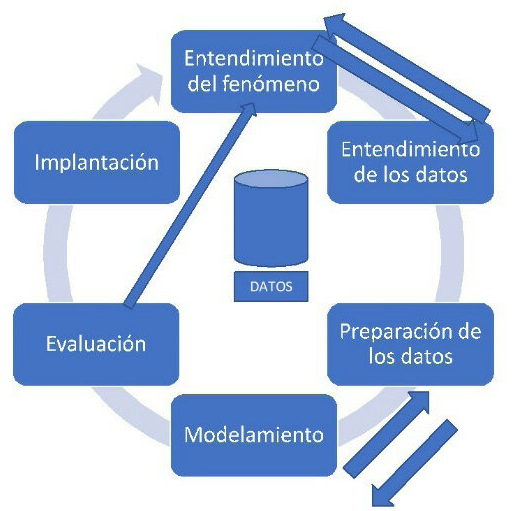
\includegraphics[width=2.6in]{Imagenes/Crips-dm} 

}

\caption{Metodología crips dm}\label{fig:unnamed-chunk-4}
\end{figure}

La metodología CRISP-DM (Cross Industry Standard Process for Data Mining) es un marco estructurado y ampliamente reconocido que guía el proceso de desarrollo de soluciones de minería de datos y modelado de datos.
Surgió en la década de 1990 como resultado de un esfuerzo colaborativo de expertos en minería de datos y análisis de datos para estandarizar y formalizar el proceso de minería de datos \textcite{Chapman2000}.

El desarrollo de CRISP-DM fue liderado por el CRISP-DM Consortium, que incluyó a empresas líderes en la industria, consultoras, universidades y organizaciones de investigación.
El objetivo era proporcionar un enfoque común y una estructura estandarizada para proyectos de minería de datos, que pudiera ser aplicable en una amplia variedad de contextos y sectores industriales \textcite{Shearer2000}.

CRISP-DM consta de seis fases principales, cada una de las cuales aborda aspectos específicos del proceso de modelado de datos:

\begin{itemize}
\item
  Comprensión del negocio (Business Understanding): En esta fase, se busca comprender los objetivos del negocio y los requisitos del proyecto de minería de datos.
  Se identifican los problemas o las oportunidades que se pretenden abordar, así como los factores críticos de éxito para el proyecto.
\item
  Comprensión de los datos (Data Understanding): Durante esta etapa, se recopilan los datos relevantes para el proyecto y se realiza un análisis exploratorio para comprender su estructura, calidad y significado.
\item
  Preparación de los datos (Data Preparation): En esta fase, se preparan los datos para su uso en el modelado mediante tareas de limpieza, integración, selección y transformación.
\item
  Modelado (Modeling): Durante esta etapa, se seleccionan y desarrollan modelos predictivos o descriptivos utilizando técnicas de minería de datos y análisis estadístico.
\item
  Evaluación (Evaluation): En esta fase, se evalúan y validan los modelos desarrollados utilizando conjuntos de datos de prueba o técnicas de validación cruzada.
\item
  Despliegue (Deployment): Finalmente, en esta etapa, se implementan los modelos en un entorno operativo y se integran en los sistemas existentes.
\end{itemize}

CRISP-DM ha sido ampliamente adoptado y utilizado en una variedad de industrias y aplicaciones \textcite{Pyle1999}, incluyendo banca, telecomunicaciones, comercio electrónico, salud, manufactura, marketing y más.

\hypertarget{planteamiento-del-problema}{%
\subsection{Planteamiento del problema}\label{planteamiento-del-problema}}

La ausencia de estimaciones precisas en el tiempo requerido para el mantenimiento correctivo en instalaciones industriales conduce a una serie de repercusiones operativas y estratégicas significativas.
Una inadecuada previsión de las horas de labor necesarias puede desencadenar una subsecuente deficiencia en la planificación y en la programación de actividades, culminando en conflictos logísticos y posibles demoras en la producción.

Los periodos de inactividad prolongados inciden directamente en la disponibilidad de maquinaria, repercutiendo en la eficiencia operativa y productiva de la planta.
Esta situación se traduce invariablemente en un incremento de los costos operacionales, ya que se acumulan horas de trabajo no contempladas inicialmente, desencadenando, en muchas ocasidades, la necesidad de recurrir a horas extra y al empleo de recursos alternativos.

A nivel financiero, la indeterminación en las labores de mantenimiento ejerce una presión considerable sobre los presupuestos establecidos, con la posibilidad de que los costos reales sobrepasen las previsiones iniciales, poniendo en juego la rentabilidad del proyecto.
Desde la perspectiva de la cadena de valor, el mantenimiento no planificado puede tener consecuencias en cadena, afectando a varios eslabones y comprometiendo compromisos comerciales previamente acordados.

La precisión en los presupuestos de proyectos de mantenimiento es vital para mantener la viabilidad financiera y la sostenibilidad de las operaciones industriales.
Una mala predicción en las horas de mantenimiento puede llevar a exceder las estimaciones presupuestarias, afectando negativamente la rentabilidad del proyecto \textcite{Wang2017}.
Asimismo, las interrupciones en el mantenimiento tienen el potencial de afectar adversamente la cadena de suministro y comprometer las relaciones con los clientes \textcite{Cheng2019}.

La moral y el bienestar del personal de mantenimiento también son áreas de preocupación significativas, donde la incertidumbre y el aumento de la carga de trabajo pueden conducir a un estrés laboral incrementado y a un deterioro en la moral del equipo \textcite{TaylorSchmidt2020}.
Además, la urgencia por reanudar la producción no debe comprometer los estándares de seguridad, ya que la seguridad del personal es de suma importancia y debe ser siempre una prioridad \textcite{GonzalezMartinez2022}.

Para abordar estos desafíos, es esencial adoptar enfoques basados en datos para mejorar la precisión de las estimaciones de tiempo de mantenimiento correctivo.
La implementación de herramientas de análisis predictivo y el uso estratégico de datos históricos son estrategias recomendadas para mejorar la planificación del mantenimiento y reducir los tiempos de inactividad no planificados \textcite{Morales2020}.

\hypertarget{proceso-previo-al-modelado}{%
\subsection{Proceso previo al modelado}\label{proceso-previo-al-modelado}}

Inicialmente, se realiza un proceso meticuloso de limpieza de la base de datos, que implica la eliminación rigurosa de valores atípicos, con el propósito de asegurar la integridad y fiabilidad del conjunto de datos.
Tras refinar la base de datos y consolidar su calidad, se procede con una fase de análisis descriptivo.
Esta etapa está orientada a adquirir una comprensión profunda del comportamiento intrínseco de las variables, así como de las interacciones potenciales que puedan existir con la variable dependiente.
Este análisis preliminar es crucial, ya que establece la fundación para la modelización predictiva posterior y el descubrimiento de insights operativos valiosos.

\hypertarget{limpiando-la-base-de-datos}{%
\subsubsection{Limpiando la base de datos}\label{limpiando-la-base-de-datos}}

El conjunto de datos que se empleará en este estudio comprende inicialmente 36,795 observaciones y 11 variables distintas, todas las cuales pertenecen al ámbito de las actividades de reparación industrial.
Este voluminoso corpus de información proporcionará una base sólida para el análisis en profundidad y la modelización de las operaciones de mantenimiento correctivo, permitiendo así un entendimiento exhaustivo de las dinámicas y los patrones subyacentes a estos procesos industriales críticos.

Las variables se describen a continuación:

\begin{itemize}
\item
  \textbf{Época del año}: Indica la época del año en que se llevo a cabo la reparación verano o invierno.
\item
  \textbf{Cumplimiento de la estrategia}: Representa la ejecución de la estrategia de mantenimiento preventivo, siendo crucial cumplir con la estrategia para evitar correctivos.
\item
  \textbf{Programa de mantenimiento}: Mensualmente se genera un programa que incluye órdenes de mantenimiento correctivas y preventivas.
  A veces, no se cumple debido a emergencias que requieren atención inmediata.
\item
  \textbf{Ready Backlog}: Indica la carga de trabajo en semanas, siendo un indicador de trabajos pendientes y la necesidad de más personal.
\item
  \textbf{HH Actv Generales}: Horas dedicadas a actividades generales como charlas HSE, capacitaciones, etc.
\item
  \textbf{HH En la Maquina}: Horas reales dedicadas a trabajos en la máquina.
  Es la variable principal a predecir, especialmente en trabajos correctivos de emergencia.
\item
  \textbf{Otras HH}: Horas dedicadas a actividades propias del mantenimiento, como apertura de permisos, aislamientos, etc.
\item
  \textbf{TipoMantenimiento}: Se clasifica en preventivo, correctivo normal y correctivo de emergencia.
  El enfoque principal es predecir el tiempo necesario para el mantenimiento correctivo, especialmente el de emergencia.
\item
  \textbf{Disciplina}: Indica los equipos de trabajo que ejecutan los mantenimientos, permitiendo predicciones por equipo.
\item
  \textbf{fe.CreadaOrden y fe.Ejecutada}: Fechas de creación y ejecución de la orden, respectivamente.
\end{itemize}

\vspace{0.2cm}

En la \textbf{tabla 1} a continuación podemos ver las primeras observaciones de nuestra base de datos

\begin{table}[H]

\caption{\label{tab:unnamed-chunk-5}Base de Datos de Mantenimiento de Equipos}
\centering
\begin{tabular}[t]{>{\raggedright\arraybackslash}p{1.5cm}>{\raggedleft\arraybackslash}p{1.5cm}>{\raggedleft\arraybackslash}p{1.5cm}>{\raggedleft\arraybackslash}p{1.5cm}>{\raggedleft\arraybackslash}p{1.5cm}>{\raggedleft\arraybackslash}p{1.5cm}>{\raggedleft\arraybackslash}p{1.5cm}>{\raggedright\arraybackslash}p{1.5cm}>{\raggedright\arraybackslash}p{1.5cm}>{}p{1.5cm}>{}p{1.5cm}>{}p{1.5cm}}
\toprule
Epoca del año & estrategia Mtto & Programa Mtto & Ready back log & HH Actv Gnerales & HH En la Maquina & Otras HH & Tipo mantenimiento & Disciplina\\
\midrule
Verano & 0.977 & 0.9459 & 5.16 & 0.4 & 6.0 & 1.0 & Correctivo & Instrumentos\\
Verano & 0.977 & 0.9459 & 5.16 & 0.4 & 2.8 & 1.0 & Correctivo & Instrumentos\\
Verano & 0.977 & 0.9459 & 5.16 & 0.3 & 1.0 & 0.0 & Correctivo & Instrumentos\\
Verano & 0.977 & 0.9459 & 5.16 & 1.7 & 17.7 & 4.0 & Correctivo & Instrumentos\\
Verano & 0.977 & 0.9459 & 5.16 & 1.3 & 15.3 & 1.2 & Correctivo & Instrumentos\\
Verano & 0.977 & 0.9459 & 5.16 & 0.9 & 1.3 & 4.8 & Correctivo & Pozoz\\
Verano & 0.977 & 0.9459 & 5.16 & 1.6 & 18.0 & 1.4 & Correctivo & Instrumentos\\
Verano & 0.977 & 0.9459 & 5.16 & 0.4 & 3.0 & 1.8 & Correctivo & Pozoz\\
Verano & 0.977 & 0.9459 & 5.16 & 1.6 & 6.6 & 3.1 & Correctivo & Instrumentos\\
Verano & 0.977 & 0.9459 & 5.16 & 2.6 & 22.5 & 5.5 & Correctivo & Instrumentos\\
\bottomrule
\end{tabular}
\end{table}

\hypertarget{preparando-los-datos-para-el-anuxe1lisis-estaduxedstico}{%
\subsubsection{Preparando los datos para el análisis estadístico}\label{preparando-los-datos-para-el-anuxe1lisis-estaduxedstico}}

Antes de proceder con la aplicación de diversas técnicas de estadística multivariante, es imperativo garantizar la adecuada preparación y limpieza de la base de datos.
Esta etapa preliminar incluye la eliminación o imputación de valores vacíos o marcados como NA, la minimización o el tratamiento de valores atípicos en las variables para evitar distorsiones en el análisis, y la evaluación de las correlaciones entre variables para identificar y mitigar posibles problemas de multicolinealidad.
Estas acciones son cruciales para asegurar la integridad y la calidad de los datos, sentando así una sólida fundación que permita la implementación efectiva y precisa de las técnicas estadísticas multivariantes.
Este proceso no solo facilita un análisis más fiable y exhaustivo, sino que también potencia la capacidad de extraer insights valiosos y significativos de los datos.

\hypertarget{eliminando-los-valores-vacuxedos}{%
\subsubsection{Eliminando los valores vacíos}\label{eliminando-los-valores-vacuxedos}}

Si los valores NA no se manejan adecuadamente, pueden introducir sesgos en el análisis de datos y el planteamiento de los modelos, ya sea porque los datos faltan tes se ignoran por completo o porque se imputan de manera incorrecta, lo que podría distorsionar las conclusiones y recomendaciones.

\begin{ROut}{Consola de R: Output~\thetcbcounter}
                \begin{footnotesize}
                \begin{verbatim} [1] 9
 \end{verbatim}
                \end{footnotesize}
                \end{ROut}

Afortunadamente en nuestra data los valores \textbf{NA} son significativamente bajos, lo que posibilita ignorarlos sin afectar considerablemente nuestros resultados.

\hypertarget{valores-atuxedpicos}{%
\subsubsection{Valores atípicos}\label{valores-atuxedpicos}}

Los datos atípicos, conocidos como outliers en inglés, son valores que se encuentran significativamente fuera del rango esperado en una variable del conjunto de datos.
En nuestro contexto pueden haber maquinas que conlleven una cantidad significativa de horas mucho mayor a las demás, para analizarlas utilizamos gráficos de caja.

Los gráficos de caja mostrados en la \textbf{figura 2} muestran estadísticas de posición clave, como los cuartiles, los valores máximos y mínimos, junto con los posibles valores atípicos.
Se nota una gran dispersión de datos en las distintas variables numéricas que estamos analizando.

\begin{figure}
\centering
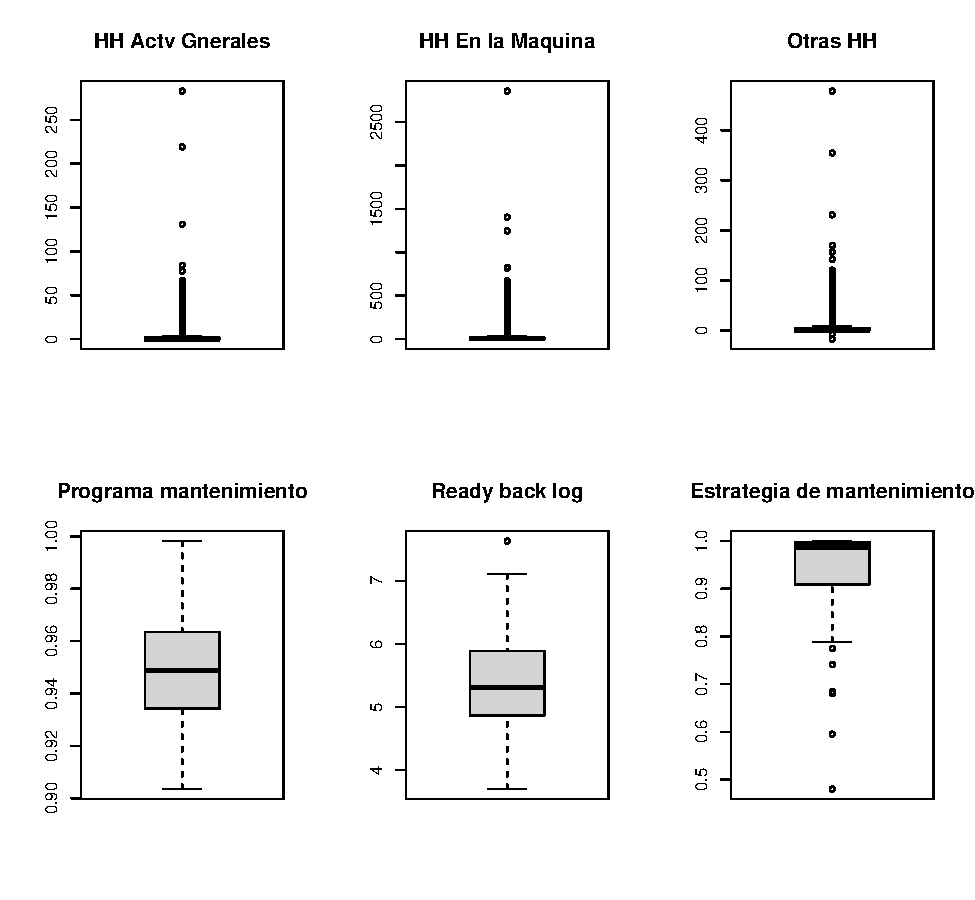
\includegraphics{trabajo_files/figure-latex/unnamed-chunk-8-1.pdf}
\caption{\label{fig:unnamed-chunk-8}Valores atípicos iniciales}
\end{figure}

HH Actv Generales: Presenta varios valores que podrían considerarse atípicos, los cuales están bastante alejados de la mediana.

HH En la Maquina: Hay menos valores atípicos comparados con la variable anterior, pero aún presenta algunos valores que son visiblemente diferentes del resto.

Otras HH: Similarmente, se muestran varios valores atípicos.

Programa Mtto: Los valores atípicos están menos dispersos que en las variables de horas; sin embargo, la mediana está más cerca del cuartil inferior, lo que podría indicar una distribución asimétrica.

Ready back log: Este boxplot también presenta valores atípicos, pero en menor cantidad en comparación con las variables de horas.

Estrategia de mantenimiento: Exhibe una distribución que parece ser más uniforme y simétrica; sin embargo, aún hay presencia de valores atípicos.

Antes de aplicar el filtro de Hampel, es importante reconocer que estos valores atípicos pueden ser indicativos de errores de medición o entrada de datos, pero también podrían representar variaciones reales dentro del proceso de mantenimiento que son importantes para entender la variabilidad del trabajo.
El filtro de Hampel reemplazará estos valores atípicos con la mediana, lo cual puede suavizar estas variaciones y presentar una vista más homogénea de los datos, pero también podría ocultar patrones o características importantes.
Por ello, siempre se debe proceder con cautela y comprender el contexto de los datos antes de aplicar cualquier método de limpieza de datos.

\textbf{¿Como tratar los valores atípicos?}

El método, conocido como \textbf{filtro de Hampel} se basa en el concepto de la mediana absoluta de las desviaciones (MAD, por sus siglas en inglés), que es una medida robusta de la variabilidad de un conjunto de datos.
La MAD se calcula como la mediana de las desviaciones absolutas de cada punto de datos con respecto a la mediana del conjunto de datos.

El filtro de Hampel es particularmente útil cuando se trabaja con datos que pueden contener valores atípicos o cuando se requiere una medida robusta de la tendencia central y la variabilidad.
Ayuda a mejorar la robustez de los análisis estadísticos al reducir el impacto de los valores extremos en los resultados.

\myequations{Filtro de Hampel}

\begin{equation}\text{Filtro de Hampel: } y_i = \begin{cases} x_i & \text{si } |x_i - \text{mediana}(X)| \leq k \times \text{MAD}(X) \\ \text{mediana} X) & \text{en otro caso} \end{cases}\end{equation}

A continuación, se detalla el proceso que describe la fórmula:

\begin{itemize}
\item
  \textbf{yi}: Representa el valor de salida para la i-ésima observación después de aplicar el Filtro de Hampel.
  Este valor puede ser el original (x\_i) si no se considera atípico, o puede ser reemplazado por la mediana del conjunto de datos si se identifica como un outlier.
\item
  \textbf{xi}: Es el valor original de la i-ésima observación en el conjunto de datos.
\item
  \textbf{Mediana(X)}: Es la mediana de todos los valores en el conjunto de datos X.
  La mediana es usada como medida de tendencia central debido a su robustez frente a valores atípicos, a diferencia de la media.
\item
  \textbf{k}: Es un factor de escala que determina el umbral de sensibilidad para identificar a un valor como atípico.
  Un valor comúnmente usado para k está en el rango de 2.5 a 3.0, aunque puede ajustarse según las necesidades específicas del análisis para controlar la tolerancia frente a las variaciones naturales en los datos.
\item
  \textbf{MAD(X)}: La Desviación Mediana Absoluta (MAD) de los valores en el conjunto de datos X.
  La MAD es una medida de dispersión que, al igual que la mediana, es menos sensible a los valores extremos en comparación con la desviación estándar.
  Proporciona una estimación de la variabilidad en torno a la mediana.
\end{itemize}

La condición \textbar x\_i - mediana(X)\textbar{} \textless= k x MAD(X) se utiliza para evaluar si un valor x\_i es un outlier.
Si la diferencia absoluta entre x\_i y la mediana de X es mayor que k veces la MAD, se considera que x\_i es un outlier y se reemplaza por la mediana del conjunto de datos; de lo contrario, se conserva el valor original x\_i.

La razón por la cual un valor se considera atípico si la diferencia absoluta entre x\_i y la mediana de X es mayor que k veces la MAD (Desviación Mediana Absoluta) se basa en la premisa de que la mayoría de los datos en un conjunto deberían agruparse cerca de una medida central ---en este caso, la mediana--- si los datos siguen una distribución relativamente simétrica o incluso si presentan cierto sesgo debido a la presencia de valores atípicos.

La mediana es una medida de tendencia central que es más robusta frente a valores atípicos que, por ejemplo, la media.
Esto significa que no se ve tan afectada por valores extremadamente altos o bajos.
La MAD, por su parte, es una medida de dispersión que indica cuán dispersos están los datos alrededor de la mediana.
Al multiplicar la MAD por un factor de escala k (comúnmente un valor entre 2.5 y 3), se establece un ``umbral'' que define lo que se considera variabilidad ``normal'' alrededor de la mediana.

Si la diferencia absoluta entre un valor particular x\_i y la mediana excede este umbral (k x MAD(X)), se asume que x\_i es tan diferente de la mayoría de los otros valores en el conjunto de datos que no se puede atribuir simplemente a la variabilidad natural de los datos.
En cambio, se considera un ``outlier'' o valor atípico, sugiriendo que podría haber sido generado por un mecanismo diferente al que produjo el resto de los datos o que podría ser el resultado de un error de medición o registro.

Al reemplazar estos valores atípicos por la mediana, se intenta mitigar su impacto en análisis posteriores, evitando que estos valores extremos distorsionen los resultados, como podría ser el caso en la estimación de parámetros de modelos estadísticos o en la construcción de predicciones.
La elección de la mediana como valor de reemplazo ayuda a mantener la estructura central de los datos sin introducir un sesgo significativo que podría resultar de utilizar, por ejemplo, la media.

Utilizando el \textbf{k} igual a 3 aplicamos el filtro de hampel en todas las variables numéricas de nuestra base de datos:

En la \textbf{figura3} se observa una reducción significa en el numero de valores atípicos, lo que indica una buena eficiencia de la técnica en eliminar los valores atípicos en la variable

\begin{figure}
\centering
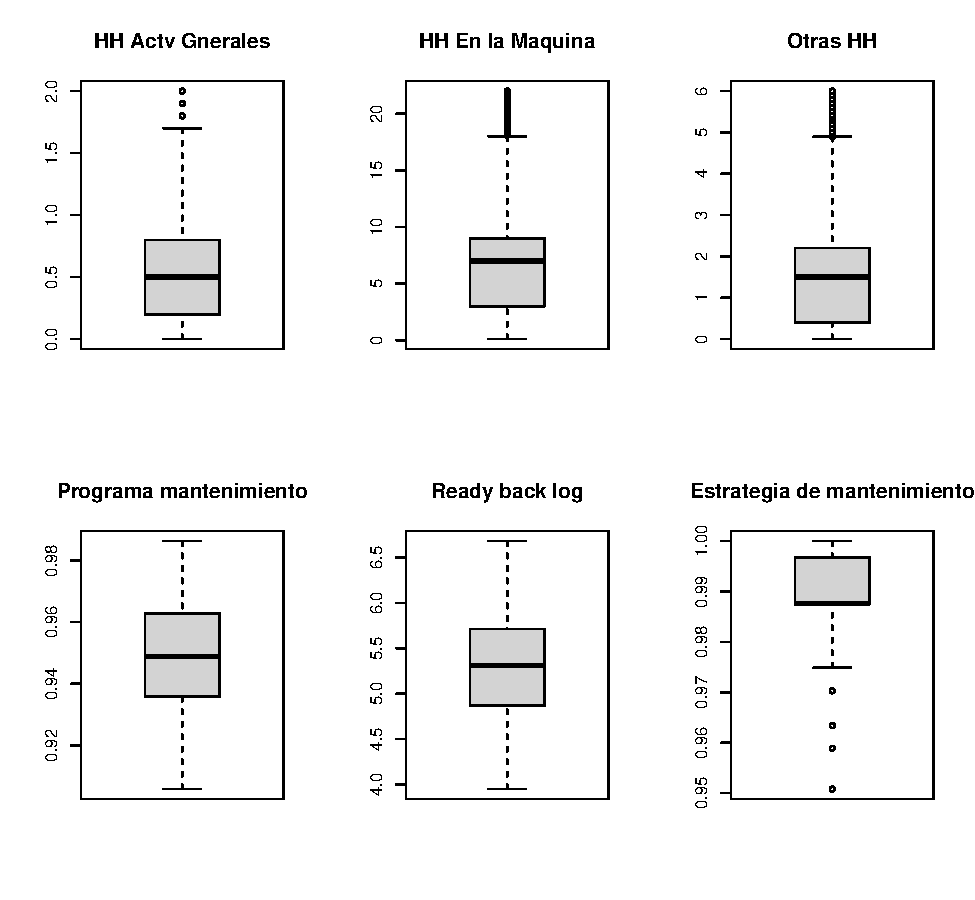
\includegraphics{trabajo_files/figure-latex/unnamed-chunk-10-1.pdf}
\caption{\label{fig:unnamed-chunk-10}Filtro de hampel aplicado}
\end{figure}

La principal diferencia visual es una reducción en la cantidad de valores atípicos visibles y una posible disminución en la longitud de los bigotes de los boxplots.
Esto implica una apariencia más limpia y posiblemente más simétrica de la distribución de los datos, reflejando una variabilidad que se ajusta más estrechamente a la mayoría de los datos, libre de las distorsiones causadas por valores extremadamente altos o bajos.

\newpage

\hypertarget{anuxe1lisis-descriptivo-de-los-datos}{%
\subsection{Análisis descriptivo de los datos}\label{anuxe1lisis-descriptivo-de-los-datos}}

En esta sección, se presenta un análisis detallado de los datos utilizados para el proyecto.
El objetivo principal es proporcionar una visión general de las características principales de la muestra, así como identificar tendencias y patrones relevantes.

\hypertarget{variables-de-tipo-cuantitativo}{%
\subsubsection{Variables de tipo cuantitativo}\label{variables-de-tipo-cuantitativo}}

\begin{table}[H]

\caption{\label{tab:unnamed-chunk-11}estadísticas descriptivas de las variables numéricas}
\centering
\begin{tabular}[t]{>{\raggedright\arraybackslash}p{1.65cm}>{\raggedleft\arraybackslash}p{1.65cm}>{\raggedleft\arraybackslash}p{1.65cm}>{\raggedleft\arraybackslash}p{1.65cm}>{\raggedleft\arraybackslash}p{1.65cm}>{\raggedleft\arraybackslash}p{1.65cm}>{\raggedleft\arraybackslash}p{1.65cm}}
\toprule
  & estrategia Mtto & Programa Mtto & Ready back log & HH Actv Gnerales & HH En la Maquina & Otras HH\\
\midrule
media & 0.9895 & 0.9492 & 5.3263 & 0.5469 & 7.1658 & 1.5905\\
mínimo & 0.9508 & 0.9058 & 3.9500 & 0.0000 & 0.1000 & 0.0000\\
cuartil 1 & 0.9876 & 0.9358 & 4.8700 & 0.2000 & 3.0000 & 0.4000\\
mediana & 0.9876 & 0.9488 & 5.3100 & 0.5000 & 7.0000 & 1.5000\\
cuartil 3 & 0.9968 & 0.9628 & 5.7100 & 0.8000 & 9.0000 & 2.2000\\
máximo & 1.0000 & 0.9863 & 6.6800 & 2.0000 & 22.0000 & 6.0000\\
varianza & 0.0001 & 0.0004 & 0.3035 & 0.2548 & 24.9059 & 2.1276\\
desviación típica & 0.0091 & 0.0199 & 0.5509 & 0.5048 & 4.9906 & 1.4586\\
coef.variación & 0.0092 & 0.0210 & 0.1034 & 0.9231 & 0.6964 & 0.9171\\
RIC & 0.0092 & 0.0270 & 0.8400 & 0.6000 & 6.0000 & 1.8000\\
asimetría & -1.9189 & -0.1608 & 0.2777 & 1.1477 & 1.0051 & 1.0706\\
curtosis & 4.9913 & -0.6679 & 0.0886 & 0.7937 & 0.3839 & 0.6339\\
moda\_1 & 0.9876 & 0.9429 & 5.3100 & 0.5000 & 7.0000 & 0.0000\\
\bottomrule
\end{tabular}
\end{table}

Al proceder con un análisis descriptivo detallado de los datos relacionados con las actividades de mantenimiento, se establece una base sólida para la construcción y formulación de modelos estadísticos avanzados.
Las estadísticas descriptivas revelan diferencias sustanciales en las escalas de medición entre las distintas variables, lo que puede conllevar a desafíos en términos de interpretación y significancia en relación con la variable objetivo.

Un aspecto notable es la variabilidad manifiesta en ciertas variables, como ``Programa Mtto'' y ``Ready back log'', donde se evidencia una dispersión considerable alrededor de la media, tal y como lo indica la magnitud de la varianza.
De igual importancia es el reconocimiento de coeficientes de variación prominentes en las variables ``HH Actv Generales'', ``HH En la Maquina'' y ``Otras HH''.
La alta variación relativa reflejada por estos coeficientes sugiere que la media no representa adecuadamente la distribución de los datos, lo cual cuestiona su utilidad como medida central para estas variables.

Estas características de los datos, como las diferencias de escala y la elevada variabilidad, podrían tener implicaciones significativas en la aplicación de modelos lineales.
En particular, los modelos que presuponen homocedasticidad y linealidad en la relación entre predictores y la variable dependiente pueden resultar inadecuados.
Por ejemplo, la influencia desmedida de variables con mayor escala puede sesgar los coeficientes estimados, llevando a interpretaciones erróneas de su relevancia en el modelo.

La precisión de las estimaciones de los coeficientes y la fiabilidad de las pruebas estadísticas subsecuentes también pueden verse afectadas por la alta variabilidad relativa.
Los modelos lineales, que son susceptibles a la influencia de valores atípicos y a una distribución anormal de los residuos, podrían no proporcionar inferencias estadísticas confiables bajo estas condiciones.

Estos problemas puede deberse a las técnicas de recolección utilizadas para recolectar los datos, según \textcite{gujarati2009basic} a medida que mejoren dichas técnicas la presencia de valores atípicos y alta varianza tenderá a disminuirse.

\hypertarget{variables-de-tipo-cualitativo}{%
\subsubsection{Variables de tipo cualitativo}\label{variables-de-tipo-cualitativo}}

\textbf{Época del año}

\begin{figure}
\centering
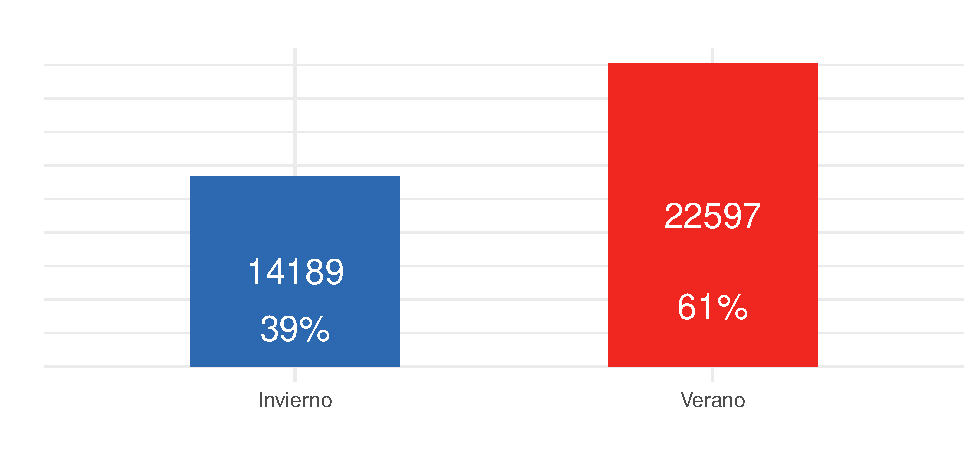
\includegraphics{trabajo_files/figure-latex/unnamed-chunk-12-1.pdf}
\caption{\label{fig:unnamed-chunk-12}Distribución de reparaciones en las épocas del año}
\end{figure}

Se nota que la mayoría de las reparaciones se llevaron a cabo durante el verano, representando un 59\% del total.
Se sugiere que el invierno podría influir en el número de horas necesarias para completar las reparaciones, lo que potencialmente aumentaría los costos y la complejidad del proceso.
De ser así esta variable se destacaría como significativa en nuestra base de datos.

\newpage

\textbf{Tipo de mantenimiento}

\begin{figure}
\centering
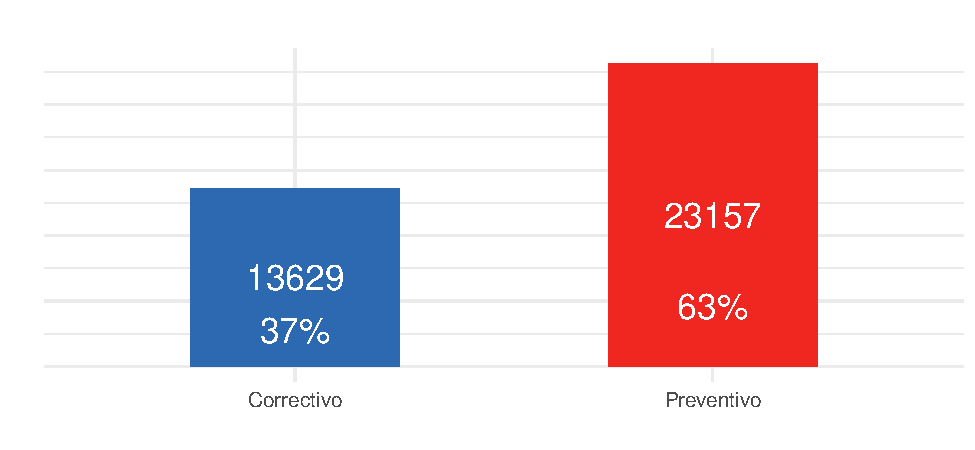
\includegraphics{trabajo_files/figure-latex/unnamed-chunk-13-1.pdf}
\caption{\label{fig:unnamed-chunk-13}Distribución de reparación según el tipo de mantenimiento}
\end{figure}

El gráfico de barras ilustra una comparativa entre las actividades de mantenimiento correctivo y preventivo.
Los modelos predictivos se centrarán en el mantenimiento correctivo, que representa el 37\% del total de las actividades, con 13,629 eventos registrados.
Este enfoque permite especializarse en anticipar las necesidades de mantenimiento correctivo, crucial para mitigar tiempos de inactividad y optimizar recursos, a pesar de ser menos frecuente que el mantenimiento preventivo.
Estos modelos tendrán un papel significativo en la mejora de la respuesta a fallos y en la eficiencia operativa general.

\newpage

\textbf{Disciplina}

\begin{figure}
\centering
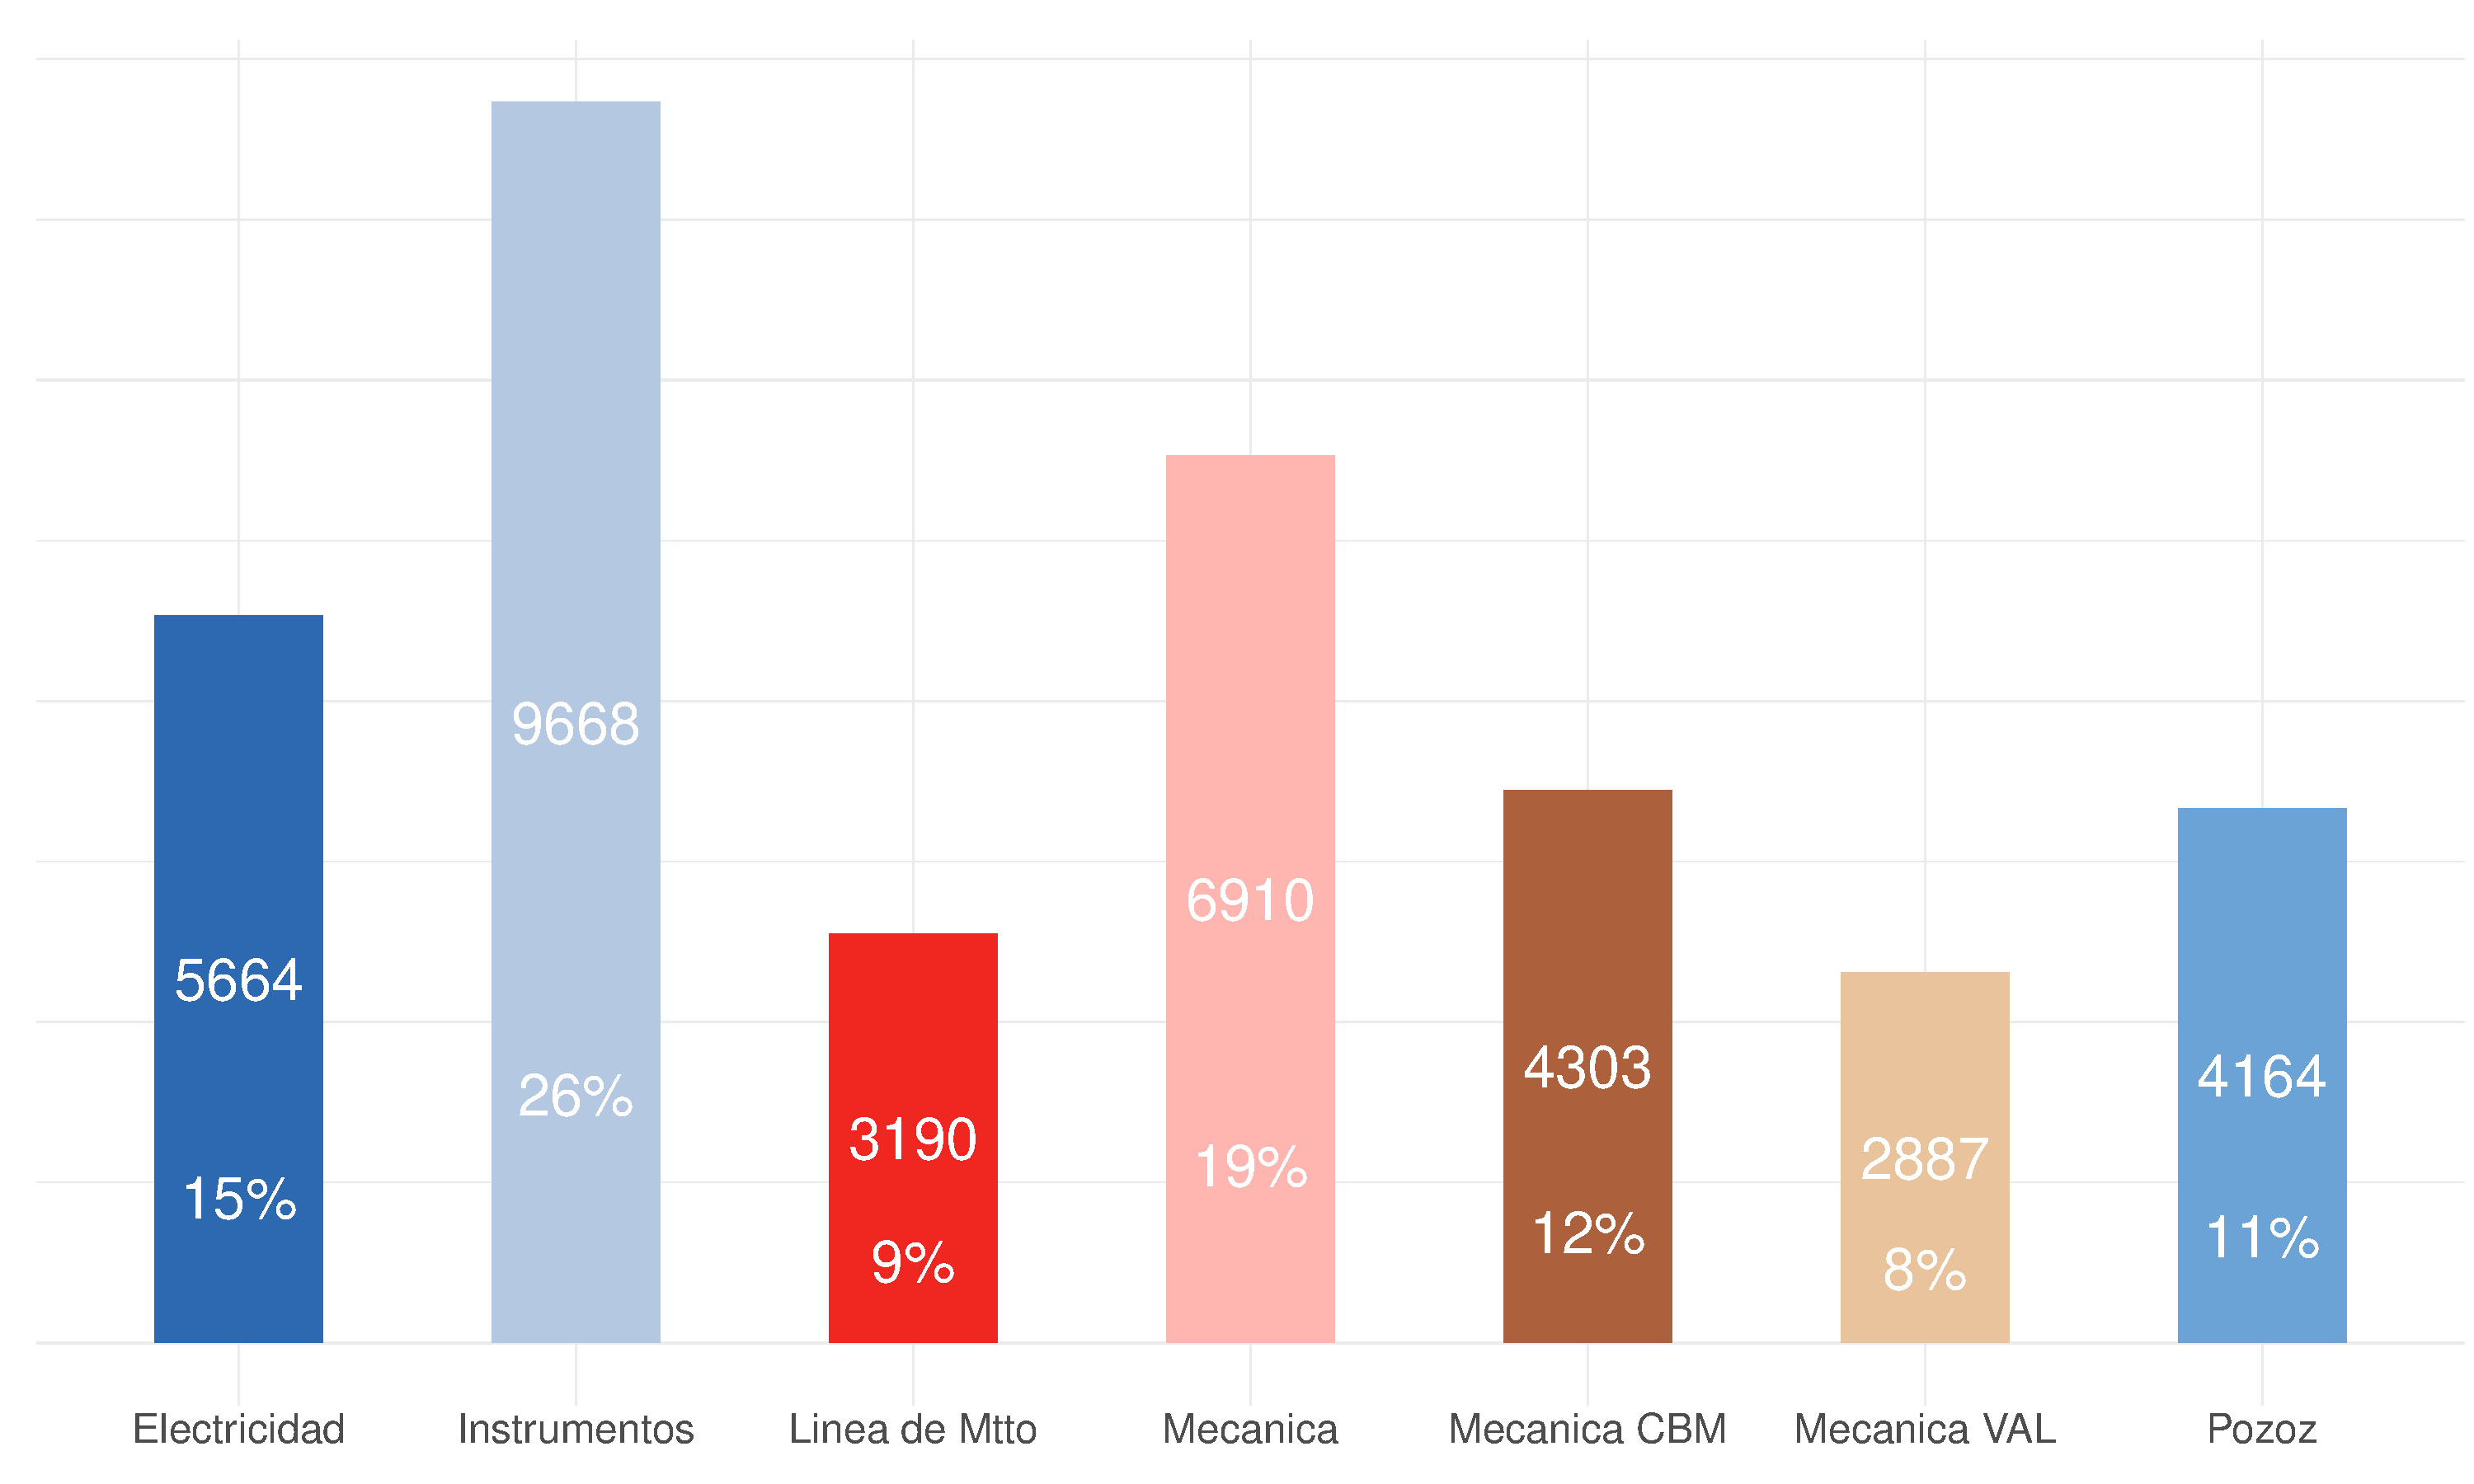
\includegraphics{trabajo_files/figure-latex/unnamed-chunk-14-1.pdf}
\caption{\label{fig:unnamed-chunk-14}Distribución de reparaciones según disciplina}
\end{figure}

\textbf{Instrumentos} es la disciplina con el mayor número de reparaciones, con un total de 9,668, lo que representa el 26\% de las reparaciones en todas las disciplinas.
Esto indica que es un área significativa de enfoque para el mantenimiento.

\textbf{Electricidad} también muestra una cantidad considerable de reparaciones, 5,664 en total, constituyendo el 15\% del total.
Aunque menor que Instrumentos, sigue siendo una parte importante de las actividades de mantenimiento.

\textbf{Línea de Mtto} (Mantenimiento) tiene 3,190 reparaciones, que es el 9\% del total, mostrando que tiene menos reparaciones en comparación con Electricidad e Instrumentos.

\textbf{Mecánica} tiene 6,910 reparaciones, un 19\% del total, lo que la coloca como una disciplina significativa pero con menos incidencias que Instrumentos.

\textbf{Mecánica CBM} (Condition Based Maintenance) cuenta con 4,303 reparaciones, representando el 12\%, sugiriendo que esta práctica proactiva de mantenimiento está razonablemente establecida.

\textbf{Mecánica VAL} (Valor Agregado de Lubricación) tiene 2,887 reparaciones, que es el 8\% del total, lo cual podría indicar que es una disciplina especializada con menos frecuencia de reparaciones.

\textbf{Pozos}, por último, muestra 4,164 reparaciones, equivalentes al 11\% del total, situándose en un punto intermedio en términos de volumen de reparaciones.

\newpage

\hypertarget{numero-de-horas-en-la-maquina-y-su-relaciuxf3n-con-otras-variables}{%
\subsubsection{Numero de horas en la maquina y su relación con otras variables}\label{numero-de-horas-en-la-maquina-y-su-relaciuxf3n-con-otras-variables}}

\textbf{Análisis de correlación}

\begin{table}[H]

\caption{\label{tab:unnamed-chunk-15}Correlación entre las variables numéricas}
\centering
\begin{tabular}[t]{>{\raggedright\arraybackslash}p{1.5cm}>{\raggedleft\arraybackslash}p{1.5cm}>{\raggedleft\arraybackslash}p{1.5cm}>{\raggedleft\arraybackslash}p{1.5cm}>{\raggedleft\arraybackslash}p{1.5cm}>{\raggedleft\arraybackslash}p{1.5cm}>{\raggedleft\arraybackslash}p{1.5cm}}
\toprule
  & estrategia Mtto & Programa Mtto & Ready back log & HH Actv Gnerales & HH En la Maquina & Otras HH\\
\midrule
estrategia Mtto & 1.00 & 0.15 & -0.15 & -0.02 & 0.00 & -0.03\\
Programa Mtto & 0.15 & 1.00 & -0.35 & -0.03 & -0.01 & -0.03\\
Ready back log & -0.15 & -0.35 & 1.00 & 0.00 & 0.00 & 0.01\\
HH Actv Gnerales & -0.02 & -0.03 & 0.00 & 1.00 & 0.46 & 0.50\\
HH En la Maquina & 0.00 & -0.01 & 0.00 & 0.46 & 1.00 & 0.44\\
Otras HH & -0.03 & -0.03 & 0.01 & 0.50 & 0.44 & 1.00\\
\bottomrule
\end{tabular}
\end{table}

Cada valor en la matriz representa el coeficiente de correlación entre dos variables específicas.
La correlación puede variar en un rango de -1 a 1:

\begin{itemize}
\item
  Un valor de 1 indica una correlación positiva perfecta, lo que significa que las dos variables están perfectamente relacionadas de manera positiva (cuando una aumenta, la otra también aumenta en proporción constante).
\item
  Un valor de -1 indica una correlación negativa perfecta, lo que significa que las dos variables están perfectamente relacionadas de manera negativa (cuando una aumenta, la otra disminuye en proporción constante).
\item
  Un valor de 0 indica que no hay correlación lineal entre las dos variables.
\end{itemize}

Para la variable dependiente (HH en la maquina) ninguna de las correlaciones con otras variables es significativa en términos de magnitud (cercana a 1 o -1).
Esto sugiere que ``HH En la Maquina'' no está fuertemente correlacionada con ninguna de las otras variables incluidas en la matriz de correlación.
Sin embargo, es importante considerar que la ausencia de correlaciones significativas no necesariamente implica una falta de relación entre las variables; podría haber otras formas de relación que no están capturadas por la correlación lineal.

\newpage

\textbf{Análisis de densidad por época del año}

\begin{figure}
\centering
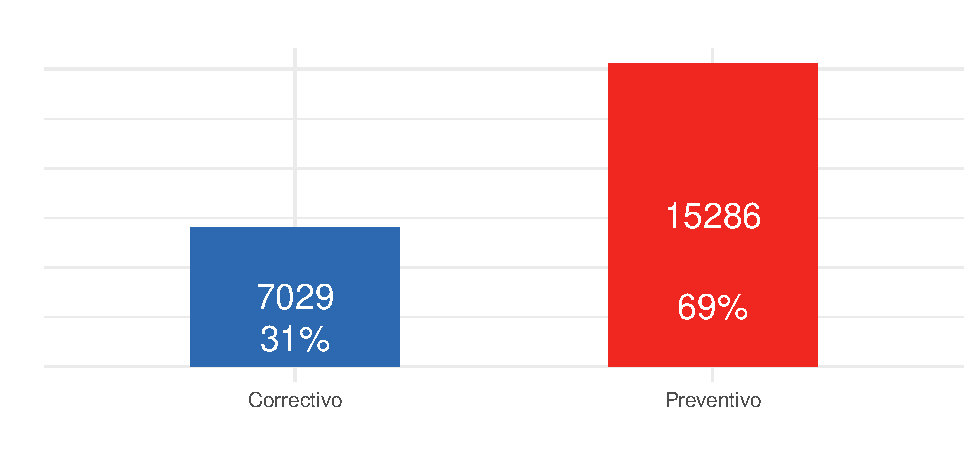
\includegraphics{trabajo_files/figure-latex/unnamed-chunk-16-1.pdf}
\caption{\label{fig:unnamed-chunk-16}Densidad de horas en la maquina por época del año}
\end{figure}

No se detectan diferencias significativas al comparar el número de horas requeridas para la reparación de la máquina durante el verano y el invierno.
Los datos revelan una variación mínima, indicando una consistencia en el tiempo de reparación independientemente de la estación.
Este patrón se mantiene constante incluso cuando el número de horas de reparación es extremadamente alto o bajo.
Estos resultados sugieren que las condiciones estacionales no ejercen un impacto significativo en el tiempo necesario para la reparación de la máquina, una conclusión que podría ser confirmada si la variable no resulta significativa en nuestros modelos.

\textbf{Análisis de densidad por tipo de mantenimiento}

\begin{figure}
\centering
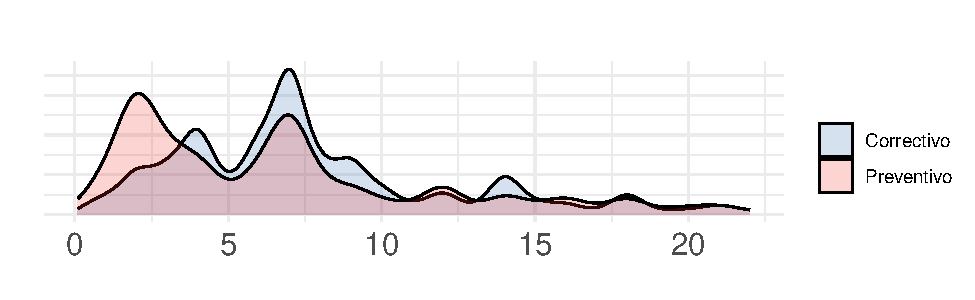
\includegraphics{trabajo_files/figure-latex/unnamed-chunk-17-1.pdf}
\caption{\label{fig:unnamed-chunk-17}Densidad de horas en la maquina por tipo de mantenimiento}
\end{figure}

Se evidencia que conforme aumenta el número de horas necesarias para la reparación de la máquina, se observa una clara tendencia en la naturaleza del mantenimiento requerido.
Los datos revelan que los mantenimientos correctivos son más frecuentes cuando se necesitan entre 5 y 10 horas para la reparación.
Este tipo de mantenimiento reactivo suele ser necesario cuando se detectan problemas más significativos que requieren una intervención inmediata para restaurar el funcionamiento adecuado de la máquina.

Por otro lado, se observa que los mantenimientos preventivos son más comunes cuando las reparaciones duran entre 0 y 5 horas.
Estos mantenimientos planificados se realizan de manera regular y sistemática para evitar la aparición de problemas mayores y mantener el equipo en óptimas condiciones de funcionamiento.
Su implementación oportuna puede reducir la necesidad de intervenciones correctivas costosas y prolongadas en el futuro.

Estos hallazgos subrayan la importancia de una gestión efectiva del mantenimiento, donde la combinación adecuada de mantenimiento preventivo y correctivo puede maximizar la disponibilidad y confiabilidad de la maquinaria, al tiempo que se minimizan los costos operativos y de reparación.

\newpage

\textbf{Análisis de densidad por disciplina}

\begin{figure}
\centering
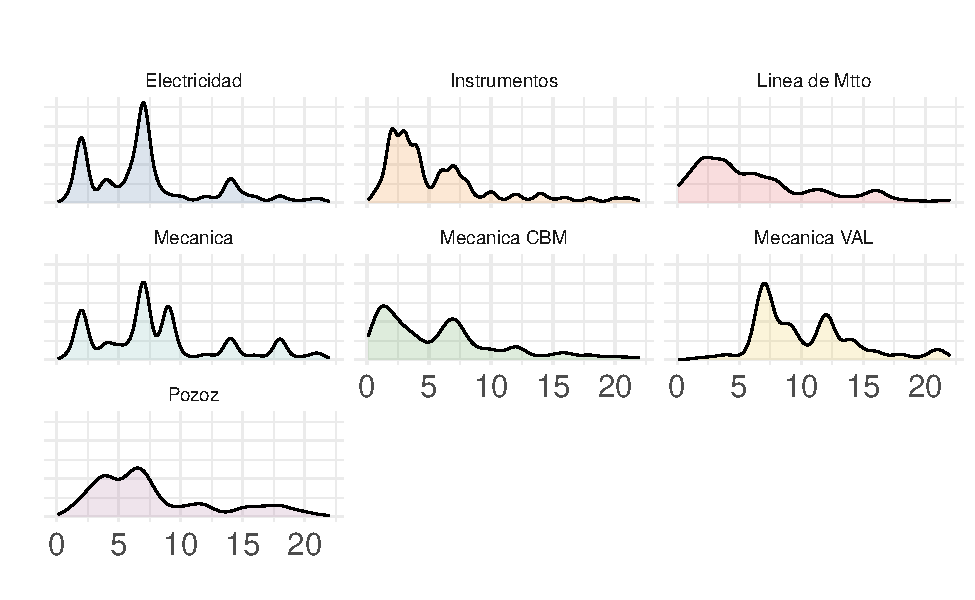
\includegraphics{trabajo_files/figure-latex/unnamed-chunk-18-1.pdf}
\caption{\label{fig:unnamed-chunk-18}Densidad de horas en la maquina por disciplina}
\end{figure}

Se pueden observar distintas densidades según el tipo de disciplina, y es evidente que en la mayoría de los casos las horas de reparación son menores a 10 horas.
Sin embargo, se destaca la disciplina VAL, donde los tiempos de reparación son significativamente mayores y se concentran en el rango de 5 a 15 horas.
Esto sugiere que esta disciplina tiende a requerir un mayor número de horas para completar las reparaciones en comparación con otras disciplinas.

\newpage

\hypertarget{planteando-los-modelos}{%
\subsection{Planteando los modelos}\label{planteando-los-modelos}}

En esta sección, nos centraremos en el análisis de los técnicas de estadística multivariante discutidos previamente en nuestro marco teórico.
Estos modelos serán aplicados en diversos contextos temporales, incluyendo el análisis diario, semanal y mensual.
El objetivo de este espacio es profundizar en la comprensión y explicación de los resultados obtenidos a partir de dichos modelos en cada una de estas escalas temporales.
Buscamos así obtener una comprensión exhaustiva de sus dinámicas, así como de los impactos que todas las variables en nuestra base de datos pueden tener en el numero de horas necesarias para reparar las maquinas.

\textbf{Base de datos agrupada de manera diaria}

En esta base de datos, organizamos la información agrupándola por día y también según la temporada del año y la disciplina de reparación.
El objetivo es calcular la media de cada variable numérica.

\textbf{Base de datos agrupada de manera semanal}

Inicialmente creamos una variable llamada ``semana'', que consiste en la combinación del año extraído de la fecha de ejecución utilizando la función \emph{year}, junto con la semana extraída de la misma fecha mediante la función \emph{week}.
Posteriormente, agrupamos los datos por esta variable, la época del año y la disciplina.

\textbf{Base de datos agrupada de manera mensual}

Inicialmente creamos una variable llamada ``mes'', que consiste en la combinación del año extraído de la fecha de ejecución utilizando la función \emph{year}, junto con el mes extraído de la misma fecha mediante la función \emph{month}.
Posteriormente, agrupamos los datos por esta variable, la época del año y la disciplina.

\textbf{Desarrollo de las predicciones}

Es crucial tener presente que nos enfrentamos a la tarea de modelar tres variaciones temporales distintas, las cuales son segmentos fundamentales de nuestro conjunto de datos que abarcan diversos aspectos temporales que buscamos pronosticar.
Al utilizar los modelos discutidos en el marco teórico, nuestro objetivo radica en comprender y anticipar cómo varían nuestras variables con cambios en las variables independientes a lo largo de estas diferentes escalas temporales.

Una vez que hemos ajustado nuestros modelos a cada una de estas variaciones temporales, se torna imperativo evaluar su rendimiento y capacidad explicativa.
Para ello, recurrimos a una serie de criterios de información, tales como el criterio de información de Akaike (AIC) o el criterio de información bayesiano (BIC), entre otros.
Estos criterios nos permiten comparar los modelos entre sí y determinar cuál de ellos se ajusta mejor a nuestros datos, teniendo en cuenta la complejidad inherente de cada modelo.

\newpage

\begin{table}[H]

\caption{\label{tab:unnamed-chunk-22}Base de Datos agrupada de manera diaria}
\centering
\resizebox{\linewidth}{!}{
\fontsize{20}{22}\selectfont
\begin{tabular}[t]{lllrrrrrr}
\toprule
fecha Ejecutada & Disciplina & Epoca del año & Cumplimiento\_Estrategia & Cumplimiento\_Programa & Ready\_Backlog & HH\_Actv\_Gnerales & HH\_En\_la\_Maquina & Otras\_HH\\
\midrule
2019-01-02 & Instrumentos & Verano & 0.98 & 0.95 & 5.16 & 0.40 & 4.40 & 1.00\\
2019-01-04 & Instrumentos & Verano & 0.98 & 0.95 & 5.16 & 0.30 & 1.00 & 0.00\\
2019-01-08 & Instrumentos & Verano & 0.98 & 0.95 & 5.16 & 0.59 & 6.73 & 1.54\\
2019-01-08 & Pozoz & Verano & 0.98 & 0.95 & 5.16 & 0.65 & 4.43 & 2.43\\
2019-01-09 & Instrumentos & Verano & 0.98 & 0.95 & 5.16 & 0.49 & 6.37 & 1.52\\
2019-01-09 & Mecanica & Verano & 0.98 & 0.95 & 5.16 & 0.50 & 5.00 & 0.60\\
2019-01-09 & Pozoz & Verano & 0.98 & 0.95 & 5.16 & 0.81 & 4.80 & 2.70\\
2019-01-11 & Electricidad & Verano & 0.98 & 0.95 & 5.16 & 0.90 & 8.80 & 1.55\\
2019-01-11 & Instrumentos & Verano & 0.98 & 0.95 & 5.16 & 0.83 & 7.71 & 2.19\\
2019-01-11 & Mecanica & Verano & 0.98 & 0.95 & 5.16 & 0.50 & 7.00 & 1.50\\
2019-01-14 & Instrumentos & Verano & 0.98 & 0.95 & 5.16 & 0.50 & 7.00 & 5.20\\
2019-01-15 & Instrumentos & Verano & 0.98 & 0.95 & 5.16 & 0.50 & 8.50 & 0.50\\
2019-01-16 & Pozoz & Verano & 0.98 & 0.95 & 5.16 & 0.40 & 1.00 & 1.60\\
2019-01-17 & Instrumentos & Verano & 0.98 & 0.95 & 5.16 & 0.80 & 3.00 & 0.60\\
2019-01-18 & Instrumentos & Verano & 0.98 & 0.95 & 5.16 & 0.80 & 2.80 & 1.10\\
\bottomrule
\end{tabular}}
\end{table}

\begin{table}[H]

\caption{\label{tab:unnamed-chunk-22}Base de Datos agrupada de manera semanal}
\centering
\resizebox{\linewidth}{!}{
\fontsize{20}{22}\selectfont
\begin{tabular}[t]{lllrrrrrr}
\toprule
semana & Disciplina & Epoca del año & Cumplimiento\_Estrategia & Cumplimiento\_Programa & Ready\_Backlog & HH\_Actv\_Gnerales & HH\_En\_la\_Maquina & Otras\_HH\\
\midrule
2019-1 & Instrumentos & Verano & 0.98 & 0.95 & 5.16 & 0.37 & 3.27 & 0.67\\
2019-10 & Pozoz & Verano & 0.99 & 0.92 & 4.67 & 0.30 & 1.80 & 1.90\\
2019-11 & Instrumentos & Verano & 0.99 & 0.92 & 4.67 & 0.20 & 0.50 & 0.00\\
2019-12 & Instrumentos & Verano & 0.99 & 0.92 & 4.67 & 1.05 & 8.00 & 1.55\\
2019-12 & Mecanica & Verano & 0.99 & 0.92 & 4.67 & 0.70 & 9.00 & 1.30\\
2019-12 & Pozoz & Verano & 0.99 & 0.92 & 4.67 & 0.60 & 3.30 & 2.20\\
2019-15 & Instrumentos & Verano & 0.99 & 0.94 & 5.65 & 0.05 & 6.10 & 0.50\\
2019-16 & Instrumentos & Verano & 0.99 & 0.94 & 5.65 & 0.57 & 8.33 & 1.93\\
2019-17 & Instrumentos & Verano & 0.99 & 0.94 & 5.65 & 0.50 & 6.50 & 0.90\\
2019-17 & Pozoz & Verano & 0.99 & 0.94 & 5.65 & 0.50 & 16.00 & 1.50\\
2019-18 & Instrumentos & Invierno & 0.99 & 0.94 & 5.96 & 0.50 & 10.70 & 1.50\\
2019-18 & Mecanica VAL & Invierno & 0.99 & 0.94 & 5.96 & 1.50 & 14.00 & 2.50\\
2019-19 & Electricidad & Invierno & 0.99 & 0.94 & 5.96 & 0.10 & 2.00 & 0.35\\
2019-19 & Pozoz & Invierno & 0.99 & 0.94 & 5.96 & 0.50 & 16.00 & 1.50\\
2019-2 & Electricidad & Verano & 0.98 & 0.95 & 5.16 & 0.90 & 8.80 & 1.55\\
\bottomrule
\end{tabular}}
\end{table}

\begin{table}[H]

\caption{\label{tab:unnamed-chunk-22}Base de Datos agrupada de manera mensual}
\centering
\resizebox{\linewidth}{!}{
\fontsize{20}{22}\selectfont
\begin{tabular}[t]{lllrrrrrr}
\toprule
mes & Disciplina & Epoca del año & Cumplimiento\_Estrategia & Cumplimiento\_Programa & Ready\_Backlog & HH\_Actv\_Gnerales & HH\_En\_la\_Maquina & Otras\_HH\\
\midrule
2019-1 & Electricidad & Verano & 0.98 & 0.95 & 5.16 & 0.74 & 10.09 & 2.39\\
2019-1 & Instrumentos & Verano & 0.98 & 0.95 & 5.16 & 0.57 & 6.65 & 1.55\\
2019-1 & Mecanica & Verano & 0.98 & 0.95 & 5.16 & 0.50 & 10.83 & 1.20\\
2019-1 & Mecanica CBM & Verano & 0.98 & 0.95 & 5.16 & 0.50 & 8.00 & 0.60\\
2019-1 & Pozoz & Verano & 0.98 & 0.95 & 5.16 & 0.69 & 4.51 & 2.49\\
2019-10 & Electricidad & Verano & 0.99 & 0.93 & 5.91 & 0.50 & 7.00 & 5.50\\
2019-10 & Instrumentos & Verano & 0.99 & 0.93 & 5.91 & 0.41 & 5.78 & 1.11\\
2019-10 & Linea de Mtto & Verano & 0.99 & 0.93 & 5.91 & 0.71 & 7.40 & 2.43\\
2019-10 & Mecanica & Verano & 0.99 & 0.93 & 5.91 & 1.45 & 15.20 & 1.35\\
2019-10 & Mecanica VAL & Verano & 0.99 & 0.93 & 5.91 & 0.00 & 12.00 & 0.00\\
2019-10 & Pozoz & Verano & 0.99 & 0.93 & 5.91 & 0.73 & 4.24 & 2.59\\
2019-11 & Electricidad & Verano & 0.99 & 0.92 & 5.89 & 1.80 & 7.00 & 5.40\\
2019-11 & Mecanica & Verano & 0.99 & 0.92 & 5.89 & 0.83 & 9.98 & 2.15\\
2019-11 & Mecanica CBM & Verano & 0.99 & 0.92 & 5.89 & 0.35 & 11.27 & 1.46\\
2019-12 & Mecanica VAL & Verano & 0.99 & 0.94 & 5.46 & 1.60 & 7.00 & 1.50\\
\bottomrule
\end{tabular}}
\end{table}

\newpage

\hypertarget{predicciuxf3n-de-manera-diaria}{%
\subsubsection{Predicción de manera diaria}\label{predicciuxf3n-de-manera-diaria}}

\textbf{Segmentación de datos}

Segmentamos los datos en un 90\% para entrenamiento y un 10\% para realizar las pruebas, lo cual deja 1295 obs para entrenar y 144 obs para probar los modelos entrenados.

\begin{table}[H]

\caption{\label{tab:unnamed-chunk-23}Base de Datos entrenamiento diario}
\centering
\resizebox{\linewidth}{!}{
\fontsize{20}{22}\selectfont
\begin{tabular}[t]{rrrrrr}
\toprule
Cumplimiento\_Estrategia & Cumplimiento\_Programa & Ready\_Backlog & HH\_Actv\_Gnerales & HH\_En\_la\_Maquina & Otras\_HH\\
\midrule
0.96 & 0.96 & 5.87 & 0.70 & 9.50 & 2.13\\
0.99 & 0.94 & 5.37 & 0.65 & 4.50 & 0.75\\
0.99 & 0.91 & 5.93 & 1.00 & 7.33 & 2.02\\
1.00 & 0.97 & 6.48 & 0.30 & 15.00 & 2.00\\
0.99 & 0.91 & 5.93 & 0.00 & 0.50 & 0.00\\
0.99 & 0.96 & 5.07 & 0.50 & 7.00 & 1.50\\
1.00 & 0.95 & 5.04 & 0.80 & 15.40 & 2.78\\
0.98 & 0.97 & 5.31 & 0.50 & 7.00 & 1.50\\
0.99 & 0.96 & 4.80 & 0.76 & 7.80 & 3.54\\
1.00 & 0.96 & 4.64 & 1.80 & 10.00 & 1.50\\
1.00 & 0.98 & 5.00 & 0.50 & 7.71 & 2.59\\
0.98 & 0.99 & 4.47 & 0.33 & 5.92 & 1.18\\
0.99 & 0.96 & 4.70 & 0.72 & 10.56 & 1.52\\
1.00 & 0.96 & 6.25 & 0.75 & 15.00 & 3.30\\
1.00 & 0.97 & 4.70 & 0.50 & 7.00 & 1.50\\
\bottomrule
\end{tabular}}
\end{table}

\begin{table}[H]

\caption{\label{tab:unnamed-chunk-23}Base de Datos de prueba diario}
\centering
\resizebox{\linewidth}{!}{
\fontsize{20}{22}\selectfont
\begin{tabular}[t]{rrrrrr}
\toprule
Cumplimiento\_Estrategia & Cumplimiento\_Programa & Ready\_Backlog & HH\_Actv\_Gnerales & HH\_En\_la\_Maquina & Otras\_HH\\
\midrule
0.98 & 0.95 & 5.16 & 0.59 & 6.73 & 1.54\\
0.98 & 0.95 & 5.16 & 0.80 & 2.80 & 1.10\\
0.99 & 0.94 & 5.82 & 1.40 & 9.00 & 2.07\\
0.99 & 0.94 & 5.82 & 0.80 & 9.00 & 1.40\\
0.99 & 0.94 & 5.65 & 0.50 & 16.00 & 1.50\\
0.99 & 0.94 & 5.96 & 0.50 & 7.00 & 1.50\\
0.99 & 0.94 & 5.78 & 0.46 & 5.88 & 1.24\\
0.99 & 0.95 & 5.75 & 0.54 & 4.20 & 2.56\\
0.99 & 0.91 & 5.17 & 0.30 & 2.00 & 0.00\\
0.99 & 0.94 & 5.88 & 0.32 & 4.88 & 0.90\\
0.99 & 0.94 & 5.88 & 0.38 & 5.50 & 0.88\\
0.99 & 0.93 & 5.91 & 0.49 & 8.55 & 1.60\\
0.99 & 0.94 & 5.39 & 0.50 & 13.30 & 2.30\\
0.99 & 0.94 & 5.39 & 0.58 & 7.25 & 2.31\\
0.99 & 0.94 & 5.39 & 0.43 & 6.79 & 2.05\\
\bottomrule
\end{tabular}}
\end{table}

\textbf{Modelos a entrenar}

En este análisis, exploramos diferentes modelos estadísticos para predecir la variable HH\_En\_la\_Maquina utilizando un conjunto de datos de entrenamiento diario llamado traindiario.

Comenzamos ajustando un modelo lineal utilizando la función lm.
Este modelo considera una relación lineal entre la variable objetivo y las variables predictoras en el conjunto de datos.

Continuamos con la exploración de modelos lineales generalizados mediante la función glm.
Estos modelos permiten modelar relaciones entre variables predictoras y la respuesta que pueden no ser lineales, y también pueden manejar variables de respuesta con distribuciones no normales.

Luego, ajustamos un modelo de regresión utilizando el método de Regresión de Soporte Vectorial (SVR).
Este modelo busca encontrar la mejor función lineal para predecir la variable objetivo HH\_En\_la\_Maquina, utilizando una función de pérdida epsilon-insensible.

Exploramos también los Bosques Aleatorios, un método de aprendizaje conjunto que construye múltiples árboles de decisión durante el entrenamiento y produce la predicción promedio de los árboles individuales.

Finalmente, ajustamos un modelo de Árboles de Decisión utilizando el método de partición recursiva (RPART), que divide iterativamente los datos en subconjuntos basados en ciertos criterios, buscando maximizar la homogeneidad dentro de los grupos resultantes.

\textbf{Que modelo elegir}

\begin{itemize}
\item
  El modelo rf (Random Forest) tiene los valores más bajos de RMSE y MSE, lo que indica que generalmente ha tenido un mejor desempeño en términos de minimizar los errores cuadrados.
  También tiene el MAE más bajo, lo que sugiere que tiene una buena precisión en términos de errores absolutos.
\item
  Los modelos lineal y glm tienen valores idénticos para todas las métricas, lo que podría indicar que tienen un rendimiento muy similar en este conjunto de datos o que podrían estar utilizando la misma fórmula subyacente para la predicción.
\item
  El svr y el arbol tienen un rendimiento ligeramente mejor que los modelos lineales en términos de RMSE y MSE, pero no superan al rf.
\end{itemize}

Estos resultados sugieren que el modelo de Random Forest es el más adecuado para los datos y el problema en cuestión, seguido por el modelo SVR, el árbol de decisión y, por último, los modelos lineales y GLM que presentan un rendimiento similar entre sí.

\begin{table}[H]

\caption{\label{tab:unnamed-chunk-25}Comparación de los modelos (base de datos diaria)}
\centering
\begin{tabular}[t]{>{\raggedleft\arraybackslash}p{2.0cm}>{\raggedleft\arraybackslash}p{2.0cm}>{\raggedleft\arraybackslash}p{2.0cm}>{\raggedright\arraybackslash}p{2.0cm}}
\toprule
RMSE & MSE & MAE & MODELO\\
\midrule
3.810062 & 14.51657 & 2.870399 & lineal\\
3.810062 & 14.51657 & 2.870399 & glm\\
3.803253 & 14.46473 & 2.821755 & svr\\
3.684542 & 13.57585 & 2.819537 & arbol\\
3.594922 & 12.92346 & 2.740100 & rf\\
\bottomrule
\end{tabular}
\end{table}

\textbf{Comparación entre valores reales y predichos}

La Tabla 10 presenta una comparativa detallada entre los valores estimados por un modelo de regresión random forest y las cifras reales observadas.

El MAE de 2.74 indica que, en promedio, las predicciones del modelo se desvían alrededor de 2.74 horas de los tiempos reales observados.
Esta discrepancia se evidencia claramente en los datos, donde las horas estimadas a menudo difieren de las horas reales dedicadas a las actividades.
Esta tendencia sugiere una posible sobrevaloración sistemática por parte del modelo, lo que lleva a la asignación excesiva o insuficiente de recursos por parte de la empresa.
Esta discrepancia media implica que, en promedio, la empresa podría estar asignando 2.75 horas más o menos de lo necesario para completar las actividades.
Esta ineficiencia en el uso de recursos, tanto económicos como humanos, subraya la necesidad de ajustar el modelo para optimizar la planificación y el despliegue de recursos.

\begin{table}[H]

\caption{\label{tab:unnamed-chunk-26}Predichos vs reales (base de datos diaria)}
\centering
\begin{tabular}[t]{>{\raggedleft\arraybackslash}p{2.0cm}>{\raggedleft\arraybackslash}p{2.0cm}>{}p{2.0cm}>{}p{2.0cm}}
\toprule
predichos & reales\\
\midrule
7.86 & 6.73\\
6.29 & 2.80\\
11.95 & 9.00\\
8.44 & 9.00\\
12.09 & 16.00\\
11.16 & 7.00\\
6.94 & 5.88\\
6.55 & 4.20\\
4.37 & 2.00\\
5.84 & 4.88\\
\bottomrule
\end{tabular}
\end{table}

\newpage

\hypertarget{predicciuxf3n-de-manera-semanal}{%
\subsubsection{Predicción de manera semanal}\label{predicciuxf3n-de-manera-semanal}}

\textbf{Segmentación de datos}

Segmentamos los datos en un 90\% para entrenamiento y un 10\% para realizar las pruebas, lo cual deja 885 obs para entrenar y 99 obs para probar los modelos entrenados.

\begin{table}[H]

\caption{\label{tab:unnamed-chunk-27}Base de Datos entrenamiento semanal}
\centering
\resizebox{\linewidth}{!}{
\fontsize{20}{22}\selectfont
\begin{tabular}[t]{rrrrrr}
\toprule
Cumplimiento\_Estrategia & Cumplimiento\_Programa & Ready\_Backlog & HH\_Actv\_Gnerales & HH\_En\_la\_Maquina & Otras\_HH\\
\midrule
1.00 & 0.97 & 4.78 & 0.81 & 12.64 & 2.15\\
1.00 & 0.95 & 4.84 & 0.25 & 3.86 & 0.40\\
0.99 & 0.95 & 5.31 & 0.78 & 5.51 & 1.99\\
0.99 & 0.96 & 4.87 & 0.20 & 8.00 & 1.00\\
0.99 & 0.94 & 5.31 & 0.97 & 7.86 & 3.16\\
0.96 & 0.99 & 4.06 & 0.40 & 8.00 & 1.35\\
0.99 & 0.96 & 4.80 & 0.68 & 9.38 & 2.10\\
0.99 & 0.93 & 5.31 & 0.67 & 5.33 & 1.63\\
1.00 & 0.96 & 5.71 & 0.96 & 6.20 & 2.72\\
0.95 & 0.94 & 6.20 & 0.89 & 7.95 & 2.07\\
0.96 & 0.96 & 5.87 & 0.58 & 7.83 & 1.43\\
0.99 & 0.94 & 5.96 & 0.50 & 16.00 & 1.50\\
0.99 & 0.92 & 4.87 & 0.64 & 9.07 & 2.77\\
1.00 & 0.93 & 4.61 & 0.58 & 5.00 & 1.90\\
0.99 & 0.95 & 5.30 & 0.50 & 10.00 & 1.10\\
\bottomrule
\end{tabular}}
\end{table}

\begin{table}[H]

\caption{\label{tab:unnamed-chunk-27}Base de Datos de prueba semanal}
\centering
\resizebox{\linewidth}{!}{
\fontsize{20}{22}\selectfont
\begin{tabular}[t]{rrrrrr}
\toprule
Cumplimiento\_Estrategia & Cumplimiento\_Programa & Ready\_Backlog & HH\_Actv\_Gnerales & HH\_En\_la\_Maquina & Otras\_HH\\
\midrule
0.98 & 0.95 & 5.16 & 0.59 & 6.73 & 1.54\\
0.98 & 0.95 & 5.16 & 0.80 & 2.80 & 1.10\\
0.99 & 0.94 & 5.82 & 1.40 & 9.00 & 2.07\\
0.99 & 0.94 & 5.82 & 0.80 & 9.00 & 1.40\\
0.99 & 0.94 & 5.65 & 0.50 & 16.00 & 1.50\\
0.99 & 0.94 & 5.96 & 0.50 & 7.00 & 1.50\\
0.99 & 0.94 & 5.78 & 0.46 & 5.88 & 1.24\\
0.99 & 0.95 & 5.75 & 0.54 & 4.20 & 2.56\\
0.99 & 0.91 & 5.17 & 0.30 & 2.00 & 0.00\\
0.99 & 0.94 & 5.88 & 0.32 & 4.88 & 0.90\\
0.99 & 0.94 & 5.88 & 0.38 & 5.50 & 0.88\\
0.99 & 0.93 & 5.91 & 0.49 & 8.55 & 1.60\\
0.99 & 0.94 & 5.39 & 0.50 & 13.30 & 2.30\\
0.99 & 0.94 & 5.39 & 0.58 & 7.25 & 2.31\\
0.99 & 0.94 & 5.39 & 0.43 & 6.79 & 2.05\\
\bottomrule
\end{tabular}}
\end{table}

\textbf{Que modelo elegir}

\begin{itemize}
\item
  El modelo rf (Random Forest) tiene los valores más bajos de RMSE y MSE, lo que indica que generalmente ha tenido un mejor desempeño en términos de minimizar los errores cuadrados.
  También tiene el MAE más bajo, lo que sugiere que tiene una buena precisión en términos de errores absolutos.
\item
  Los modelos lineal y glm tienen valores idénticos para todas las métricas, lo que podría indicar que tienen un rendimiento muy similar en este conjunto de datos o que podrían estar utilizando la misma fórmula subyacente para la predicción.
\item
  El svr y el arbol tienen un rendimiento ligeramente mejor que los modelos lineales en términos de RMSE y MSE, pero no superan al rf.
\end{itemize}

Estos resultados sugieren que el modelo de Random Forest es el más adecuado para los datos y el problema en cuestión, seguido por el modelo SVR, el árbol de decisión y, por último, los modelos lineales y GLM que presentan un rendimiento similar entre sí.

\begin{table}[H]

\caption{\label{tab:unnamed-chunk-29}Comparación de los modelos (base de datos semana)}
\centering
\begin{tabular}[t]{>{\raggedleft\arraybackslash}p{2.0cm}>{\raggedleft\arraybackslash}p{2.0cm}>{\raggedleft\arraybackslash}p{2.0cm}>{\raggedright\arraybackslash}p{2.0cm}}
\toprule
RMSE & MSE & MAE & MODELO\\
\midrule
3.291756 & 10.835660 & 2.481877 & lineal\\
3.291756 & 10.835660 & 2.481877 & glm\\
3.313117 & 10.976742 & 2.480234 & svr\\
3.365729 & 11.328129 & 2.574055 & arbol\\
3.117299 & 9.717555 & 2.380497 & rf\\
\bottomrule
\end{tabular}
\end{table}

\textbf{Comparación entre valores reales y predichos}

La Tabla 14 presenta una comparativa detallada entre los valores estimados por un modelo de regresión random forest y las cifras reales observadas.

El MAE de 2.38 indica que, en promedio, las predicciones del modelo se desvían alrededor de 2.38 horas de los tiempos reales observados.

\begin{table}[H]

\caption{\label{tab:unnamed-chunk-30}Predichos vs reales (base de datos semanal)}
\centering
\begin{tabular}[t]{>{\raggedleft\arraybackslash}p{2.0cm}>{\raggedleft\arraybackslash}p{2.0cm}>{}p{2.0cm}>{}p{2.0cm}}
\toprule
predichos & reales\\
\midrule
5.12 & 3.27\\
5.01 & 0.50\\
3.90 & 6.10\\
12.18 & 14.00\\
6.84 & 6.41\\
8.95 & 6.00\\
5.72 & 5.53\\
7.65 & 16.90\\
6.93 & 6.71\\
6.42 & 8.00\\
\bottomrule
\end{tabular}
\end{table}

\newpage

\hypertarget{predicciuxf3n-de-manera-mensual}{%
\subsubsection{Predicción de manera mensual}\label{predicciuxf3n-de-manera-mensual}}

\textbf{Segmentación de datos}

Segmentamos los datos en un 90\% para entrenamiento y un 10\% para realizar las pruebas, lo cual deja 157 obs para entrenar y 18 obs para probar los modelos entrenados.

\begin{table}[H]

\caption{\label{tab:unnamed-chunk-31}Base de Datos entrenamiento mensual}
\centering
\resizebox{\linewidth}{!}{
\fontsize{20}{22}\selectfont
\begin{tabular}[t]{rrrrrr}
\toprule
Cumplimiento\_Estrategia & Cumplimiento\_Programa & Ready\_Backlog & HH\_Actv\_Gnerales & HH\_En\_la\_Maquina & Otras\_HH\\
\midrule
0.99 & 0.92 & 4.87 & 0.89 & 7.51 & 2.22\\
0.99 & 0.92 & 5.89 & 0.35 & 11.27 & 1.46\\
1.00 & 0.97 & 4.70 & 0.44 & 5.99 & 0.79\\
0.98 & 0.99 & 4.47 & 0.50 & 14.50 & 1.43\\
0.95 & 0.94 & 6.20 & 0.84 & 10.96 & 2.58\\
0.96 & 0.99 & 4.06 & 0.56 & 9.83 & 2.17\\
0.99 & 0.96 & 4.55 & 0.83 & 9.47 & 2.09\\
1.00 & 0.98 & 4.75 & 0.60 & 8.16 & 2.23\\
0.98 & 0.97 & 5.31 & 0.69 & 10.88 & 1.82\\
1.00 & 0.94 & 5.63 & 0.48 & 6.39 & 0.94\\
0.99 & 0.93 & 5.31 & 0.79 & 5.14 & 2.75\\
0.99 & 0.93 & 6.68 & 0.70 & 8.06 & 2.02\\
0.99 & 0.96 & 5.07 & 0.85 & 10.00 & 2.61\\
1.00 & 0.97 & 4.70 & 0.70 & 9.83 & 1.85\\
0.99 & 0.95 & 4.88 & 0.74 & 10.39 & 1.76\\
\bottomrule
\end{tabular}}
\end{table}

\begin{table}[H]

\caption{\label{tab:unnamed-chunk-31}Base de Datos de prueba mensual}
\centering
\resizebox{\linewidth}{!}{
\fontsize{20}{22}\selectfont
\begin{tabular}[t]{rrrrrr}
\toprule
Cumplimiento\_Estrategia & Cumplimiento\_Programa & Ready\_Backlog & HH\_Actv\_Gnerales & HH\_En\_la\_Maquina & Otras\_HH\\
\midrule
0.99 & 0.94 & 5.82 & 0.44 & 8.33 & 1.46\\
0.99 & 0.94 & 5.82 & 1.36 & 8.40 & 1.78\\
0.99 & 0.94 & 5.37 & 0.42 & 5.59 & 1.92\\
0.99 & 0.94 & 5.37 & 0.66 & 4.24 & 1.74\\
1.00 & 0.96 & 5.71 & 0.72 & 10.39 & 2.30\\
0.99 & 0.94 & 5.39 & 0.55 & 7.57 & 1.36\\
0.99 & 0.94 & 5.39 & 0.74 & 10.30 & 2.31\\
0.99 & 0.91 & 5.93 & 0.14 & 2.72 & 0.50\\
0.99 & 0.93 & 6.68 & 0.82 & 9.77 & 2.37\\
0.99 & 0.95 & 5.31 & 0.95 & 5.75 & 3.92\\
0.95 & 0.94 & 6.20 & 0.86 & 7.86 & 2.24\\
1.00 & 0.97 & 6.48 & 0.79 & 9.79 & 2.06\\
1.00 & 0.97 & 6.48 & 0.71 & 5.94 & 2.15\\
1.00 & 0.95 & 4.84 & 0.78 & 4.94 & 1.82\\
1.00 & 0.97 & 5.28 & 0.29 & 5.72 & 0.46\\
\bottomrule
\end{tabular}}
\end{table}

\textbf{Que modelo elegir}

\begin{itemize}
\item
  El modelo rf (Random Forest) tiene los valores más bajos de RMSE y MSE, lo que indica que generalmente ha tenido un mejor desempeño en términos de minimizar los errores cuadrados.
  También tiene el MAE más bajo, lo que sugiere que tiene una buena precisión en términos de errores absolutos.
\item
  Los modelos lineal y glm tienen valores idénticos para todas las métricas, lo que podría indicar que tienen un rendimiento muy similar en este conjunto de datos o que podrían estar utilizando la misma fórmula subyacente para la predicción.
\item
  El svr y el arbol tienen un rendimiento ligeramente mejor que los modelos lineales en términos de RMSE y MSE, pero no superan al rf.
\end{itemize}

Estos resultados sugieren que el modelo de Random Forest es el más adecuado para los datos y el problema en cuestión, seguido por el modelo SVR, el árbol de decisión y, por último, los modelos lineales y GLM que presentan un rendimiento similar entre sí.

\begin{table}[H]

\caption{\label{tab:unnamed-chunk-33}Comparación de los modelos (base de datos mensual)}
\centering
\begin{tabular}[t]{>{\raggedleft\arraybackslash}p{2.0cm}>{\raggedleft\arraybackslash}p{2.0cm}>{\raggedleft\arraybackslash}p{2.0cm}>{\raggedright\arraybackslash}p{2.0cm}}
\toprule
RMSE & MSE & MAE & MODELO\\
\midrule
2.422662 & 5.869292 & 2.092053 & lineal\\
2.422662 & 5.869292 & 2.092053 & glm\\
2.573291 & 6.621829 & 2.127786 & svr\\
2.497598 & 6.237998 & 2.107832 & arbol\\
2.376143 & 5.646056 & 1.981288 & rf\\
\bottomrule
\end{tabular}
\end{table}

\textbf{Comparación entre valores reales y predichos}

La Tabla 18 presenta una comparativa detallada entre los valores estimados por un modelo de regresión random forest y las cifras reales observadas.

El MAE de 2.38 indica que, en promedio, las predicciones del modelo se desvían alrededor de 2.38 horas de los tiempos reales observados.

\begin{table}[H]

\caption{\label{tab:unnamed-chunk-34}Predichos vs reales (base de datos mensual)}
\centering
\begin{tabular}[t]{>{\raggedleft\arraybackslash}p{2.0cm}>{\raggedleft\arraybackslash}p{2.0cm}>{}p{2.0cm}>{}p{2.0cm}}
\toprule
predichos & reales\\
\midrule
8.83 & 8.33\\
11.57 & 8.40\\
8.57 & 5.59\\
8.43 & 4.24\\
8.12 & 10.39\\
8.00 & 7.57\\
8.70 & 10.30\\
4.76 & 2.72\\
8.31 & 9.77\\
9.00 & 5.75\\
\bottomrule
\end{tabular}
\end{table}

\newpage

\hypertarget{conclusiones}{%
\section{Conclusiones}\label{conclusiones}}

\hypertarget{resultados}{%
\subsection{Resultados}\label{resultados}}

Al examinar los resultados del modelo de Random Forest, se destaca su desempeño, especialmente en el análisis mensual, donde registra un MAE de 1.981288 horas.
Este valor más bajo indica una mayor precisión en la predicción del tiempo requerido para realizar mantenimientos correctivos en un periodo prolongado.
La consistencia en este rendimiento sugiere que el modelo es especialmente eficaz cuando se consideran períodos extensos.

La ventaja del análisis mensual puede atribuirse a varios factores.
En primer lugar, al agrupar datos en un periodo más largo, se pueden eliminar ciertas fluctuaciones o variaciones aleatorias que podrían afectar las predicciones diarias o semanales.
Además, al analizar tendencias durante un mes, el modelo puede capturar patrones más estables y significativos en los datos, lo que resulta en predicciones más precisas.

Por lo tanto, al planificar actividades de mantenimiento a largo plazo, el análisis mensual proporcionado por el modelo de Random Forest emerge como la opción más confiable y precisa.

El modelo de Random Forest sobresale entre otros enfoques de modelado, como modelos lineales, GLM (Modelos Lineales Generalizados), SVR (Máquinas de Vectores de Soporte para Regresión) y árboles de decisión, por varias razones:

Robustez frente a datos complejos: Mientras que los modelos lineales y GLM son eficientes bajo ciertas suposiciones sobre la linealidad y la independencia de las variables, los datos en la práctica suelen ser más complejos, exhibiendo relaciones no lineales que podrían limitar la capacidad de estos modelos para capturar patrones subyacentes.
En contraste, el modelo de Random Forest, al emplear múltiples árboles de decisión y combinar sus predicciones, puede manejar con mayor eficacia esta complejidad inherente en los datos.

Capacidad para manejar multicolinealidad y características no lineales: En escenarios donde las variables predictoras están altamente correlacionadas o muestran relaciones no lineales con la variable objetivo, los modelos lineales y GLM pueden enfrentar dificultades para capturar estas relaciones de manera efectiva.
Por el contrario, los árboles de decisión, incluido el modelo de Random Forest, poseen la capacidad inherente de manejar multicolinealidad y relaciones no lineales sin necesidad de preprocesamiento adicional de datos.

Regularización implícita: A diferencia de los modelos lineales y SVR, que a menudo requieren técnicas de regularización para evitar el sobreajuste, el modelo de Random Forest tiende a ser menos propenso a este fenómeno debido a la naturaleza de ensamblaje de múltiples árboles de decisión.
Esto implica que el modelo puede generalizar mejor a datos no vistos, lo que se traduce en predicciones más robustas y confiables.

Manejo efectivo de variables categóricas y no lineales: Los árboles de decisión, incluido Random Forest, son intrínsecamente capaces de manejar variables categóricas sin necesidad de transformaciones adicionales, lo que simplifica el proceso de modelado y reduce la necesidad de preprocesamiento de datos.
Además, estos modelos pueden identificar interacciones no lineales entre variables predictoras, permitiendo la captura de patrones más complejos en los datos.

\newpage

\hypertarget{dificultades}{%
\subsection{Dificultades}\label{dificultades}}

La predicción del tiempo necesario para reparar máquinas es fundamental en la gestión eficiente del mantenimiento industrial.
Sin embargo, este proceso presenta una serie de desafíos que deben abordarse para desarrollar modelos predictivos precisos y útiles.

Uno de los principales desafíos es la variabilidad inherente en el tiempo de reparación, que puede ser influenciada por una multitud de factores, como la complejidad de la falla, la disponibilidad de repuestos y la experiencia del técnico \textcite{montgomery2012introduction}.
Además, la falta de datos completos sobre reparaciones anteriores puede dificultar la construcción de modelos predictivos robustos.

La relación entre las variables predictoras y el tiempo de reparación también puede ser no lineal, lo que requiere el uso de técnicas avanzadas de modelado, como modelos no lineales y de regresión robustos \textcite{gelman2013bayesian}.
Además, los efectos aleatorios, como la variabilidad entre técnicos o máquinas, pueden introducir una fuente adicional de variabilidad en el modelo.

Para abordar estos desafíos, se pueden emplear una variedad de enfoques estadísticos.
Por ejemplo, los modelos mixtos o jerárquicos pueden capturar efectos aleatorios y variabilidad no observada \textcite{agresti2015foundations}, mientras que las técnicas de imputación de datos pueden ayudar a manejar la falta de datos completos.
Asimismo, los métodos de validación cruzada y las técnicas de selección de modelos pueden utilizarse para evaluar y comparar diferentes modelos y determinar el más adecuado para un conjunto de datos dado.

A pesar de los desafíos, el modelado preciso del tiempo de reparación de máquinas puede tener un impacto significativo en la eficiencia operativa y la planificación del mantenimiento, lo que hace que valga la pena abordar estos desafíos con determinación y utilizando enfoques estadísticos adecuados.

\hypertarget{trabajos-futuros}{%
\subsection{Trabajos futuros}\label{trabajos-futuros}}

El tema de la predicción del tiempo de reparación mediante modelos estadísticos es una área de investigación en constante evolución que tiene aplicaciones importantes en diversos campos, desde la industria manufacturera hasta el mantenimiento de equipos de infraestructura.
Uno de los principales objetivos de esta investigación es desarrollar modelos predictivos precisos que puedan estimar con precisión el tiempo necesario para completar una reparación en función de una serie de variables predictoras.

Los avances en este campo han permitido la aplicación de una amplia gama de técnicas estadísticas, desde modelos de regresión lineal hasta métodos más sofisticados como el aprendizaje automático y la inteligencia artificial.
Estos modelos pueden tener en cuenta una variedad de factores que pueden influir en el tiempo de reparación, como la complejidad de la avería, la disponibilidad de piezas de repuesto, las habilidades del personal de mantenimiento y las condiciones ambientales.

Por ejemplo, en un estudio reciente realizado por \textcite{smith2020predicting}, se utilizó un modelo de regresión lineal para predecir el tiempo de reparación de equipos industriales en función de la edad del equipo, la gravedad de la avería y la experiencia del técnico de mantenimiento.
Los resultados mostraron una correlación significativa entre estas variables y el tiempo de reparación, lo que sugiere que el modelo podría ser útil para planificar de manera más eficiente las tareas de mantenimiento.

Además, investigaciones como la de \textcite{liu2019predicting} han explorado el uso de técnicas de aprendizaje automático, como los árboles de decisión y las redes neuronales, para predecir el tiempo de reparación de vehículos en función de datos históricos de mantenimiento.
Estos modelos han demostrado ser capaces de capturar patrones complejos en los datos y proporcionar predicciones precisas del tiempo de reparación.

\newpage

\hypertarget{referencias}{%
\section*{Referencias}\label{referencias}}
\addcontentsline{toc}{section}{Referencias}

\AtNextBibliography{\normalsize}
\printbibliography[heading=none]
\normalsize

\def\printbibliography{}

\begin{center}\rule{0.5\linewidth}{0.5pt}\end{center}

\hypertarget{apuxe9ndices}{%
\section*{APÉNDICES}\label{apuxe9ndices}}
\addcontentsline{toc}{section}{APÉNDICES}

\hypertarget{appendix-apuxe9ndice}{%
\appendix}


\hypertarget{paquetes-list}{%
\subsection*{\texorpdfstring{\emph{Apéndice A.} Paquetes de R usados para crear este documento}{Apéndice A. Paquetes de R usados para crear este documento}}\label{paquetes-list}}
\addcontentsline{toc}{subsection}{\emph{Apéndice A.} Paquetes de R usados para crear este documento}

Los archivos y el código necesarios para crear este documento están disponibles en el siguiente github:

A continuación se muestra la información del sistema, versión de R, y lista de paquetes usados con sus versiones:

\textbf{R version 4.2.3 (2023-03-15 ucrt)}

\textbf{Platform:} x86\_64-w64-mingw32/x64 (64-bit)

\textbf{attached base packages:}
\emph{stats}, \emph{graphics}, \emph{grDevices}, \emph{utils}, \emph{datasets}, \emph{methods} and \emph{base}

\textbf{other attached packages:}
\emph{randomForest(v.4.7-1.1)}, \emph{Metrics(v.0.1.4)}, \emph{e1071(v.1.7-13)}, \emph{rpart(v.4.1.19)}, \emph{ggthemes(v.5.1.0)}, \emph{MuMIn(v.1.47.5)}, \emph{lme4(v.1.1-32)}, \emph{Matrix(v.1.5-3)}, \emph{car(v.3.1-2)}, \emph{carData(v.3.0-5)}, \emph{lmtest(v.0.9-40)}, \emph{zoo(v.1.8-11)}, \emph{DT(v.0.27)}, \emph{readxl(v.1.4.2)}, \emph{lubridate(v.1.9.2)}, \emph{forcats(v.1.0.0)}, \emph{stringr(v.1.5.0)}, \emph{dplyr(v.1.1.1)}, \emph{purrr(v.1.0.1)}, \emph{readr(v.2.1.4)}, \emph{tidyr(v.1.3.0)}, \emph{tibble(v.3.2.1)}, \emph{ggplot2(v.3.4.2)}, \emph{tidyverse(v.2.0.0)}, \emph{kableExtra(v.1.3.4)} and \emph{knitr(v.1.42)}

\textbf{loaded via a namespace (and not attached):}
\emph{nlme(v.3.1-162)}, \emph{webshot(v.0.5.4)}, \emph{httr(v.1.4.5)}, \emph{tools(v.4.2.3)}, \emph{utf8(v.1.2.3)}, \emph{R6(v.2.5.1)}, \emph{colorspace(v.2.1-0)}, \emph{withr(v.2.5.0)}, \emph{tidyselect(v.1.2.0)}, \emph{gridExtra(v.2.3)}, \emph{compiler(v.4.2.3)}, \emph{cli(v.3.6.1)}, \emph{rvest(v.1.0.3)}, \emph{xml2(v.1.3.3)}, \emph{labeling(v.0.4.2)}, \emph{bookdown(v.0.38)}, \emph{scales(v.1.2.1)}, \emph{proxy(v.0.4-27)}, \emph{systemfonts(v.1.0.4)}, \emph{digest(v.0.6.31)}, \emph{minqa(v.1.2.5)}, \emph{rmarkdown(v.2.21)}, \emph{svglite(v.2.1.1)}, \emph{pkgconfig(v.2.0.3)}, \emph{htmltools(v.0.5.5)}, \emph{fastmap(v.1.1.1)}, \emph{highr(v.0.10)}, \emph{htmlwidgets(v.1.6.2)}, \emph{rlang(v.1.1.0)}, \emph{rstudioapi(v.0.14)}, \emph{shiny(v.1.7.4)}, \emph{farver(v.2.1.1)}, \emph{generics(v.0.1.3)}, \emph{magrittr(v.2.0.3)}, \emph{Rcpp(v.1.0.10)}, \emph{munsell(v.0.5.0)}, \emph{fansi(v.1.0.4)}, \emph{abind(v.1.4-5)}, \emph{lifecycle(v.1.0.3)}, \emph{stringi(v.1.7.12)}, \emph{yaml(v.2.3.7)}, \emph{estadistica(v.0.2.3)}, \emph{MASS(v.7.3-58.2)}, \emph{grid(v.4.2.3)}, \emph{promises(v.1.2.0.1)}, \emph{shinydashboard(v.0.7.2)}, \emph{lattice(v.0.20-45)}, \emph{splines(v.4.2.3)}, \emph{pander(v.0.6.5)}, \emph{hms(v.1.1.3)}, \emph{pillar(v.1.9.0)}, \emph{boot(v.1.3-28.1)}, \emph{stats4(v.4.2.3)}, \emph{glue(v.1.6.2)}, \emph{evaluate(v.0.20)}, \emph{data.table(v.1.14.8)}, \emph{png(v.0.1-8)}, \emph{vctrs(v.0.6.1)}, \emph{nloptr(v.2.0.3)}, \emph{tzdb(v.0.3.0)}, \emph{httpuv(v.1.6.9)}, \emph{cellranger(v.1.1.0)}, \emph{gtable(v.0.3.3)}, \emph{xfun(v.0.42)}, \emph{mime(v.0.12)}, \emph{xtable(v.1.8-4)}, \emph{later(v.1.3.0)}, \emph{class(v.7.3-21)}, \emph{viridisLite(v.0.4.1)}, \emph{timechange(v.0.2.0)} and \emph{ellipsis(v.0.3.2)}

\hypertarget{paquetes-cit}{%
\subsection*{\texorpdfstring{\emph{Apéndice B.} Citas y referencias de paquetes de R}{Apéndice B. Citas y referencias de paquetes de R}}\label{paquetes-cit}}
\addcontentsline{toc}{subsection}{\emph{Apéndice B.} Citas y referencias de paquetes de R}

Es crucial citar los paquetes de R que se utilicen en un proyecto.
Para encontrar la cita recomendada por los autores de un paquete en particular, se puede emplear la función \emph{citation()} de R.
Basta con proporcionar el nombre del paquete deseado como argumento entre comillas para acceder a la información de cita correspondiente.

\begin{thebibliography}{99}

\bibitem{tidyverse}
Hadley Wickham et al. \emph{tidyverse: Easily Install and Load the 'Tidyverse'}. 2020. R package version 1.3.0. \url{https://CRAN.R-project.org/package=tidyverse}

\bibitem{readxl}
Hadley Wickham and Jennifer Bryan. \emph{readxl: Read Excel Files}. 2019. R package version 1.3.1. \url{https://CRAN.R-project.org/package=readxl}

\bibitem{DT}
Yihui Xie et al. \emph{DT: A Wrapper of the JavaScript Library 'DataTables'}. 2020. R package version 0.18. \url{https://CRAN.R-project.org/package=DT}

\bibitem{lmtest}
Torsten Hothorn and Achim Zeileis. \emph{lmtest: Testing Linear Regression Models}. 2020. R package version 0.9-38. \url{https://CRAN.R-project.org/package=lmtest}

\bibitem{car}
John Fox et al. \emph{car: Companion to Applied Regression}. 2021. R package version 3.0-12. \url{https://CRAN.R-project.org/package=car}

\end{thebibliography}

\printbibliography

\end{document}
